\documentclass[a4paper, twoside]{report}

%% Language and font encodings
\usepackage[portuges]{babel}
\usepackage[utf8x]{inputenc}
\usepackage[T1]{fontenc}
\usepackage{verbatim}
\usepackage{float}
%% Sets page size and margins
\usepackage[a4paper,top=3cm,bottom=2cm,left=3cm,right=3cm,marginparwidth=1.75cm, paperwidth=210mm,textwidth=160mm]{geometry}
%% Useful packages
\usepackage{amsmath}
\usepackage{graphicx}
\usepackage[colorinlistoftodos]{todonotes}
\usepackage[colorlinks=true, allcolors=blue]{hyperref}
\usepackage{multirow}

\title{ConfiguraFácil}
\author{André Gonçalo Castro Peixoto, A82260\\
        Henrique José Carvalho Faria, A82200\\
        Luís Filipe da Costa Cunha, A83099\\
        Miguel Ângelo Moreira Ramos Brandão, A82349}
% Update supervisor and other title stuff in title/title.tex


\begin{document}

\begin{titlepage}

\newcommand{\HRule}{\rule{\linewidth}{0.5mm}} % Defines a new command for the horizontal lines, change thickness here

%----------------------------------------------------------------------------------------
%	LOGO SECTION
%----------------------------------------------------------------------------------------
\begin{center}
    
\includegraphics[width=5cm]{title/logoEEUM.jpg}\\[1cm] % Include a department/university logo - this will require the graphicx package
\end{center}
%----------------------------------------------------------------------------------------

\center % Center everything on the page

%----------------------------------------------------------------------------------------
%	HEADING SECTIONS
%----------------------------------------------------------------------------------------

\textsc{\LARGE Universidade do Minho}\\[1.5cm] % Name of your university/college
\textsc{\Large Mestrado Integrado em Engenharia Informática}\\[0.5cm] % Major heading such as course name
\textsc{\large Desenvolvimento de Sistemas de Software}\\[1.1cm] % Minor heading such as course title

%----------------------------------------------------------------------------------------
%	TITLE SECTION
%----------------------------------------------------------------------------------------
\makeatletter
\HRule \\[0.4cm]
{ \huge \bfseries \@title}\\[0.1cm] % Title of your document
\HRule \\[1.5cm]
 
%----------------------------------------------------------------------------------------
%	AUTHOR SECTION
%----------------------------------------------------------------------------------------

% \begin{minipage}{0.4\textwidth}
% \begin{flushleft} \large
% \emph{Author:}\\
% \@author % Your name
% \end{flushleft}
% \end{minipage}
% ~
% \begin{minipage}{0.4\textwidth}
% \begin{flushright} \large
% \emph{Supervisor:} \\
% Prof. Lily Smith \\[1.2em] % Supervisor's Name
% \emph{Second Marker:} \\
% Dr. Adam Smith % second marker's name
% \end{flushright}
% \end{minipage}\\[2cm]
% \makeatother

% If you don't want a supervisor, uncomment the two lines below and remove the section above
\Large 
%\emph{Autores:}
%\\
\@author\\[3cm] % Your name

%----------------------------------------------------------------------------------------
%	DATE SECTION
%----------------------------------------------------------------------------------------
\vspace*{\fill}

{\large \today}\\[2cm] % Date, change the \today to a set date if you want to be precise

%\vfill % Fill the rest of the page with whitespace

\end{titlepage}

\tableofcontents


\chapter{Introdução}
    O objetivo deste trabalho é analisar e modelar uma aplicação \textit{desktop} de gestão e comunicação entre um stand e uma fábrica e, posteriormente, codificar e executar esta mesma aplicação. Para isto, o software deve:
\begin{itemize}
    \item permitir que um funcionário de stand, junto do cliente, consiga configurar e enviar uma encomenda de um novo carro para a fábrica;
    \item ter pacotes de configuração predefinidos e com desconto;
    \item propor a melhor configuração possível perante um limite máximo a gastar;
    \item verificar se um componente obriga à colocação de mais componentes; 
    \item permitir guardar e retomar uma configuração pendente;
    \item indicar os carros a serem produzidos por ordem de chegada de configurações;
    \item permitir ao funcionário de fábrica atualizar o stock de componentes.
\end{itemize}

\noindent
Além disto, o software \underline{não} deve:

\begin{itemize}
    \item permitir que componentes incompatíveis sejam incluídos na mesma encomenda;
    \item permitir que uma encomenda seja enviada sem possuir todos os componentes obrigatórios;
    \item permitir que uma encomenda seja enviada quando não existe um número de componentes suficiente em stock para a satisfazer;
\end{itemize}

\noindent
Neste relatório, ilustraremos o processo de que usamos para planear e, posteriormente, programar a aplicação, tomando sempre em consideração os requisitos enunciados acima.
    
\chapter{Modelação}
    \section{Modelo de domínio}

\begin{figure}[h]
    \centering
    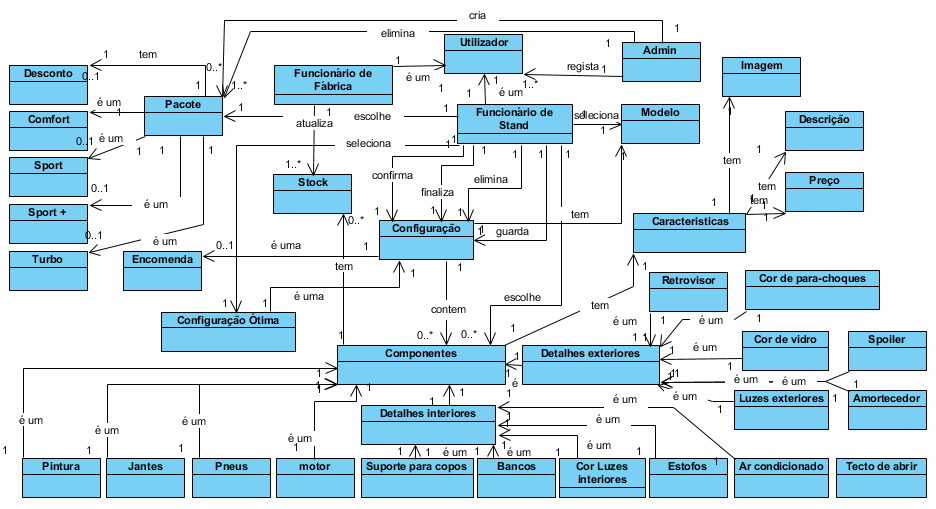
\includegraphics[width=\textwidth]{analise_de_requisitos/img/modelo_de_dominio.png}
    \caption{Modelo de domínio}
    \label{fig:modelo_de_dominio}
\end{figure}


Neste trabalho temos duas classes principais: o funcionário de fábrica e o funcionário de stand. Estes fazem ambos parte da classe \textit{utilizador}, que por sua vez são registados pelo administrador do sistema sempre que necessário adicionar um novo empregado.

O funcionário de stand trata de escolher os componentes das configurações, assim como as confirmações necessárias (se existe stock suficiente) e finalizações (envio de encomendas). Também pode guardar ou eliminar as configurações que pretender, desde que estas não tenham sido finalizadas. Adicionalmente, o funcionário seleciona o modelo do carro a encomendar sempre que iniciar uma nova configuração, pois os componentes diferem de modelo para modelo. Para além da seleção de pacotes inteiros (com desconto), tem a possibilidade de selecionar uma “configuração ótima” que preenche, também automaticamente, os componentes que fazem o melhor uso do limite de dinheiro do respetivo cliente.

Aos funcionários de fábrica, a aplicação permite modificar o stock de cada componente, que atualiza automaticamente no sistema para configurações futuras.

Por fim, para além de puder registar funcionários, o administrador do sistema pode também criar mais pacotes e eliminar os que já existem, conforme as necessidades da fábrica.

\clearpage
    \section{Modelo de \textit{uses cases}}

\begin{figure}
    \centering
    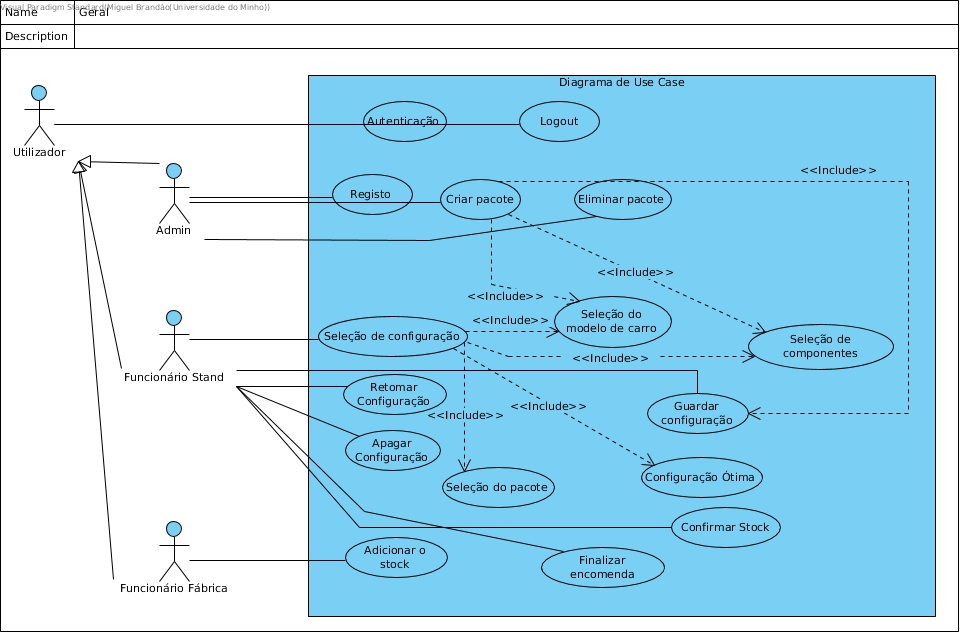
\includegraphics[width=\textwidth]{analise_de_requisitos/img/use_cases/diagrama_de_use_case.jpg}
    \caption{Diagrama de \textit{use cases}}
    \label{fig:diagrama_de_use_cases}
\end{figure}



Com o diagrama de \textit{use cases} representado pela figura \ref{fig:diagrama_de_use_cases}, podemos observar que temos 16 \textit{use cases} no total, sendo apenas dois deles comuns a todos os utilizadores (autenticação e \textit{logout}). Por vezes, foi necessário alterar os \textit{use cases}, conforme fomos construindo o programa e aumentando o nosso conhecimento do problema. Os \textit{use cases} estão especificados abaixo, com uma pequena descrição da sua função e uma referência para uma especificação no método tabular:
\begin{itemize}
    \item Autenticação (fig: \ref{fig:uc_autenticacao}): o utilizador entra no sistema;
    \item Logout (fig: \ref{fig:uc_logout}): o utilizador sai do sistema;
    \item Registo (fig: \ref{fig:uc_registo}): o administrador regista outro utilizador (quer seja funcionário de fábrica, funcionário de stand ou outro administrador);
    \item Criar Pacote (fig: \ref{fig:uc_criar_pacote}): o administrador cria um novo pacote de configuração que ainda não existe no sistema;
    \item Eliminar Pacote (fig: \ref{fig:uc_eliminar_pacote}): o administrador elimina um pacote de configuração existente no sistema;
    \item Retomar Configuração (fig: \ref{fig:uc_retormar_configuracao}): o funcionário de stand continua a configuração que tinha guardado anteriormente;
    \item Apagar Configuração (fig: \ref{fig:uc_apagar_configuracao}): o funcionário de stand apaga uma configuração guardada (se existir);
    \item Seleção de Configuração (fig: \ref{fig:uc_selecao_configuracao}):  o funcionário do stand cria uma nova configuração;
    \item Seleção do Modelo de Carro (fig: \ref{fig:uc_selecao_modelo_carro}): o funcionário de stand seleciona o tipo de carro que o cliente pretende encomendar;
    \item Seleção do Pacote (fig: \ref{fig:uc_selecao_pacote}): o funcionário de stand seleciona um pacote de configuração disponível a encomendar;
    \item Confirmar stock (fig: \ref{fig:uc_confirmar_stock}): a aplicação verifica se existe stock de todos os componentes pretendidos
    \item Configuração Ótima (fig: \ref{fig:uc_configuracao_otima}): o funcionário de stand insere o montante limite que o cliente está disposta a pagar e o sistema preenche automaticamente a melhor escolha;
    \item Seleção de Componentes (fig: \ref{fig:uc_selecao_componentes}): o funcionário de stand preenche manualmente cada componente para uma configuração personalizada;
    \item Guardar Configuração (fig: \ref{fig:uc_guardar_configuracao}): o funcionário de stand guarda a configuração do cliente no sistema para ser retomada no futuro;
   % \item Confirmar Encomenda: o funcionário de stand confirma que existe stock na fábrica para satisfazer a configuração do cliente;
    \item Finalizar Encomenda (fig: \ref{fig:uc_finalizar_encomenda}): o funcionário de stand finaliza a encomenda depois de ter sido confirmada (é enviada para a \textit{queue} de encomendas na fábrica);
    \item Adicionar o Stock (fig: \ref{fig:uc_adicionar_stock}): o funcionário de fábrica adiciona ou remove componentes manualmente no sistema.
\end{itemize}

\begin{figure}[ht]
    \centering
    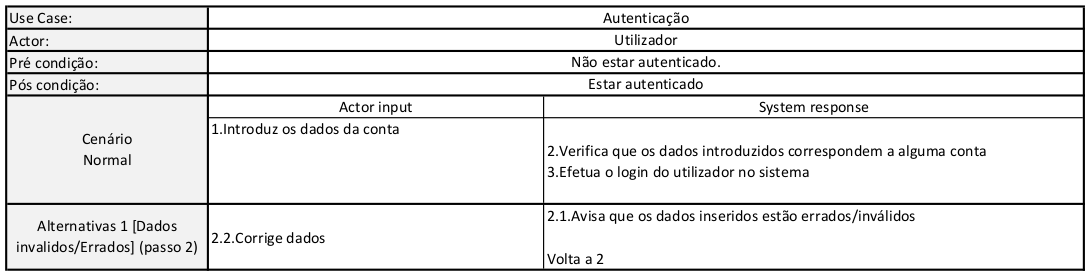
\includegraphics[width=\textwidth]{analise_de_requisitos/img/use_cases/autenticacao.png}
    \caption{\textit{Use case}: Autenticação}
    \label{fig:uc_autenticacao}
\end{figure}

\begin{figure}[ht]
    \centering
    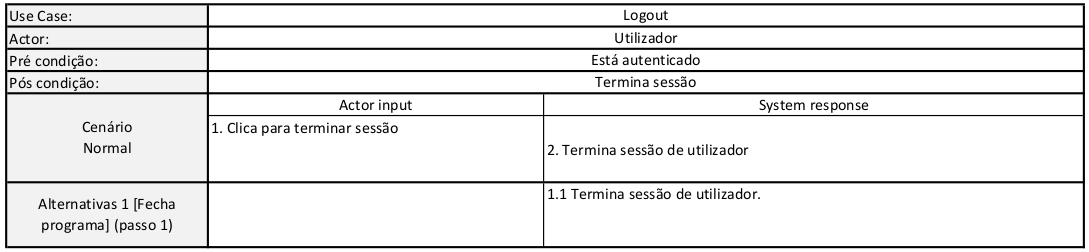
\includegraphics[width=\textwidth]{analise_de_requisitos/img/use_cases/logout.png}
    \caption{\textit{Use case}: Logout}
    \label{fig:uc_logout}
\end{figure}

\begin{figure}[ht]
    \centering
    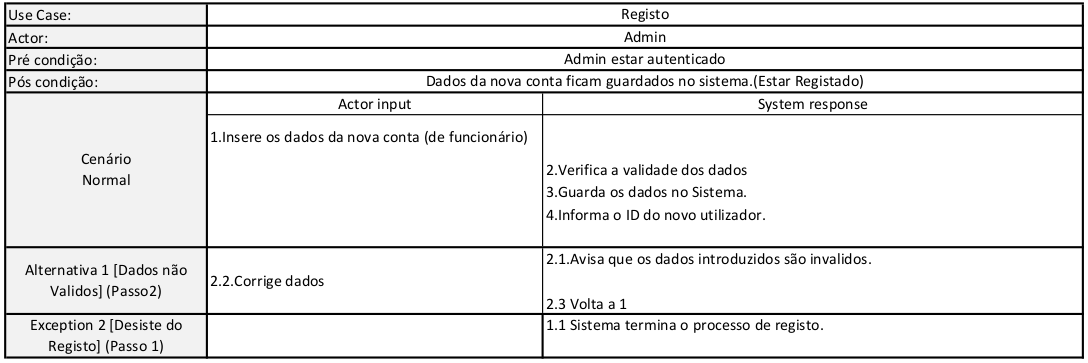
\includegraphics[width=\textwidth]{analise_de_requisitos/img/use_cases/registo.png}
    \caption{\textit{Use case}: Registo}
    \label{fig:uc_registo}
\end{figure}

\begin{figure}[ht]
    \centering
    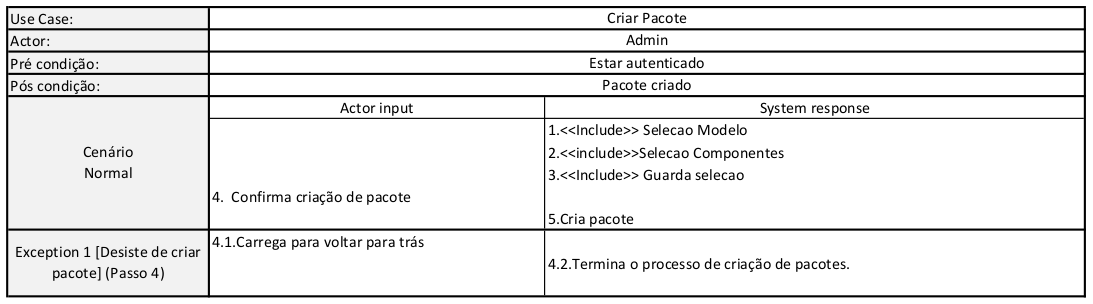
\includegraphics[width=\textwidth]{analise_de_requisitos/img/use_cases/criar_pacote.png}
    \caption{\textit{Use case}: Criar pacote}
    \label{fig:uc_criar_pacote}
\end{figure}

\begin{figure}[ht]
    \centering
    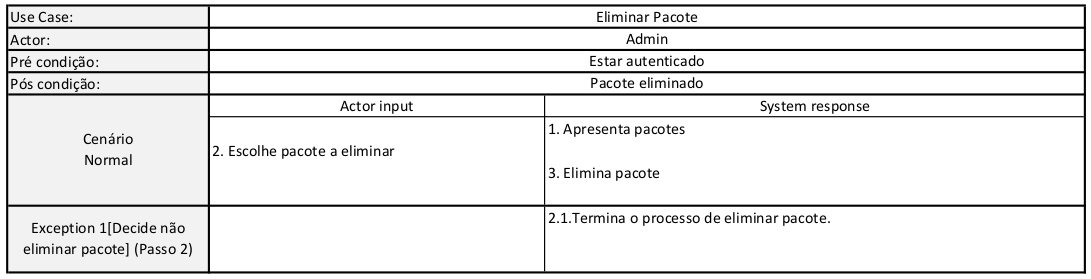
\includegraphics[width=\textwidth]{analise_de_requisitos/img/use_cases/eliminar_pacote.png}
    \caption{\textit{Use case}: Eliminar pacote}
    \label{fig:uc_eliminar_pacote}
\end{figure}

\begin{figure}[ht]
    \centering
    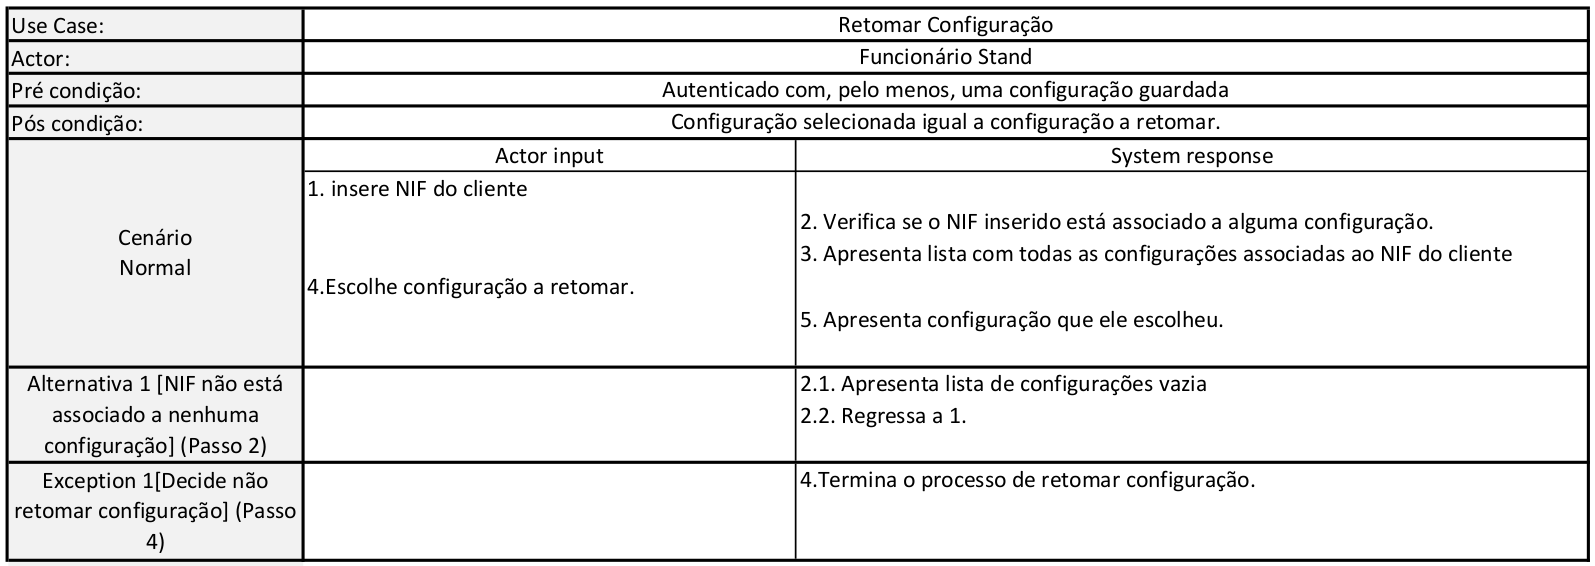
\includegraphics[width=\textwidth]{analise_de_requisitos/img/use_cases/retomar_configuracao.png}
    \caption{\textit{Use case}: Retomar configuração}
    \label{fig:uc_retormar_configuracao}
\end{figure}

\begin{figure}[ht]
    \centering
    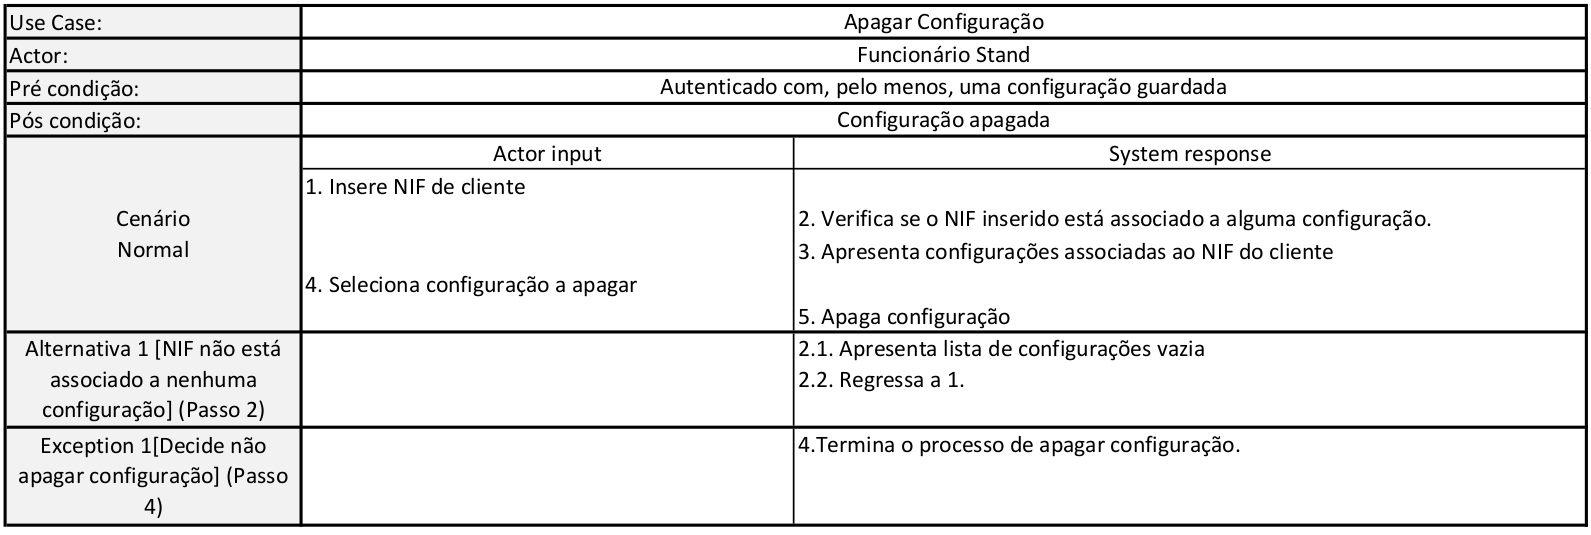
\includegraphics[width=\textwidth]{analise_de_requisitos/img/use_cases/apagar_configuracao.png}
    \caption{\textit{Use case}: Apagar configuração}
    \label{fig:uc_apagar_configuracao}
\end{figure}

\begin{figure}[ht]
    \centering
    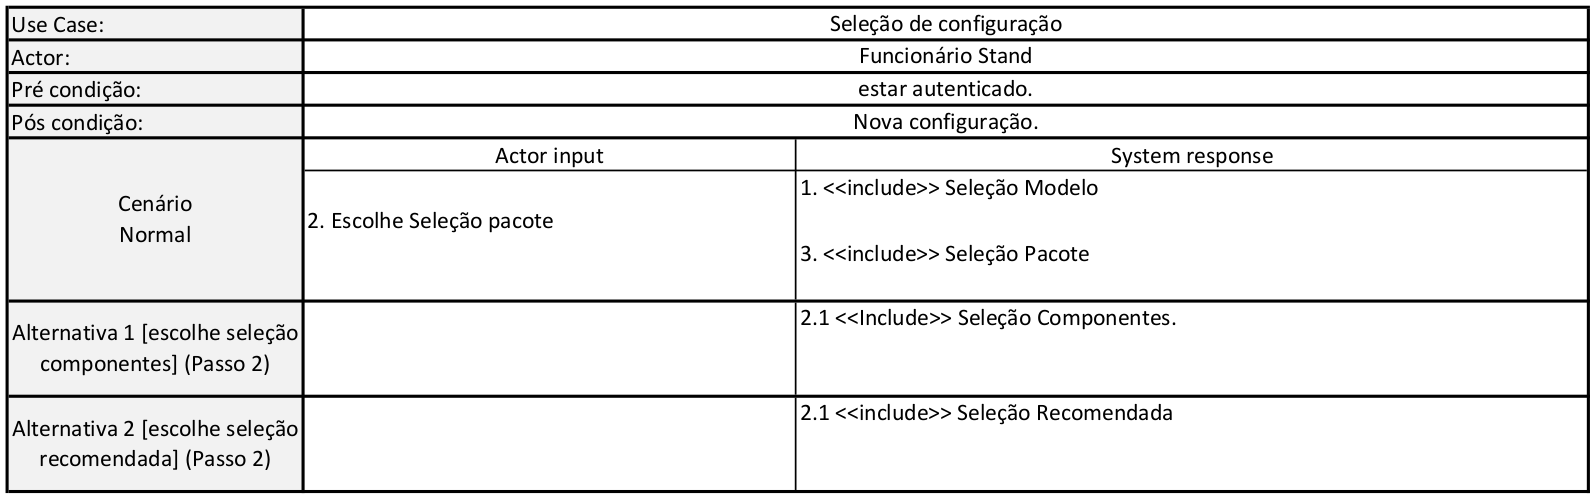
\includegraphics[width=\textwidth]{analise_de_requisitos/img/use_cases/selecao_configuracao.png}
    \caption{\textit{Use case}: Seleção de configuração}
    \label{fig:uc_selecao_configuracao}
\end{figure}

\begin{figure}[ht]
    \centering
    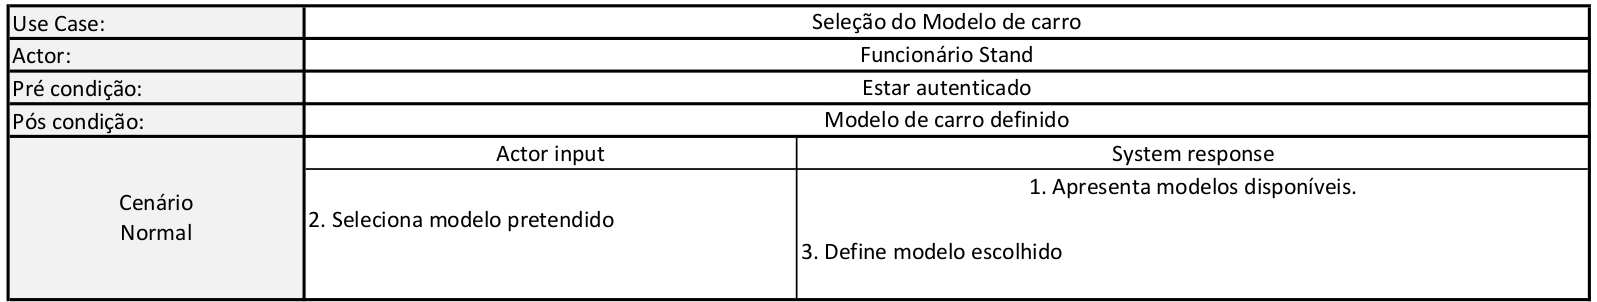
\includegraphics[width=\textwidth]{analise_de_requisitos/img/use_cases/selecao_modelo_carro.png}
    \caption{\textit{Use case}: Seleção do Modelo de Carro}
    \label{fig:uc_selecao_modelo_carro}
\end{figure}

\begin{figure}[ht]
    \centering
    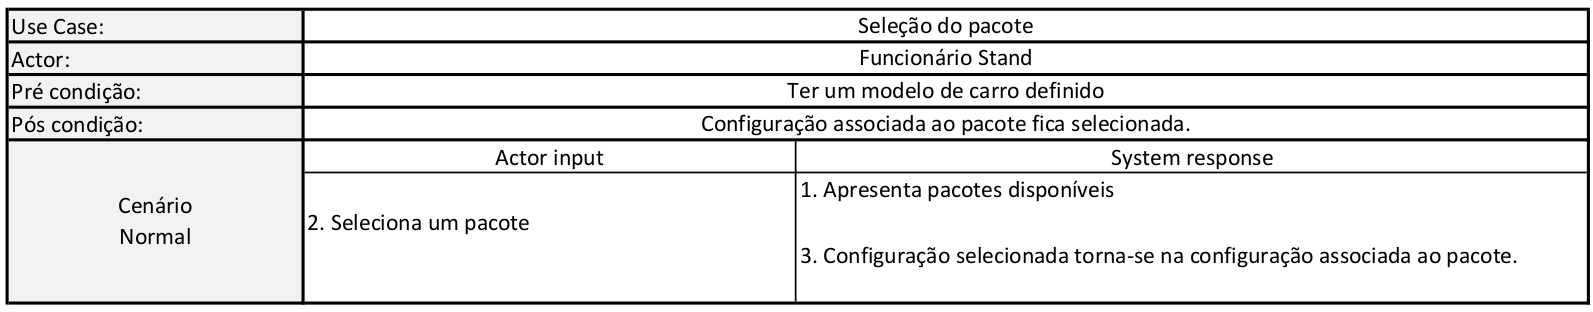
\includegraphics[width=\textwidth]{analise_de_requisitos/img/use_cases/selecao_pacote.png}
    \caption{\textit{Use case}: Seleção do pacote}
    \label{fig:uc_selecao_pacote}
\end{figure}

\begin{figure}[ht]
    \centering
    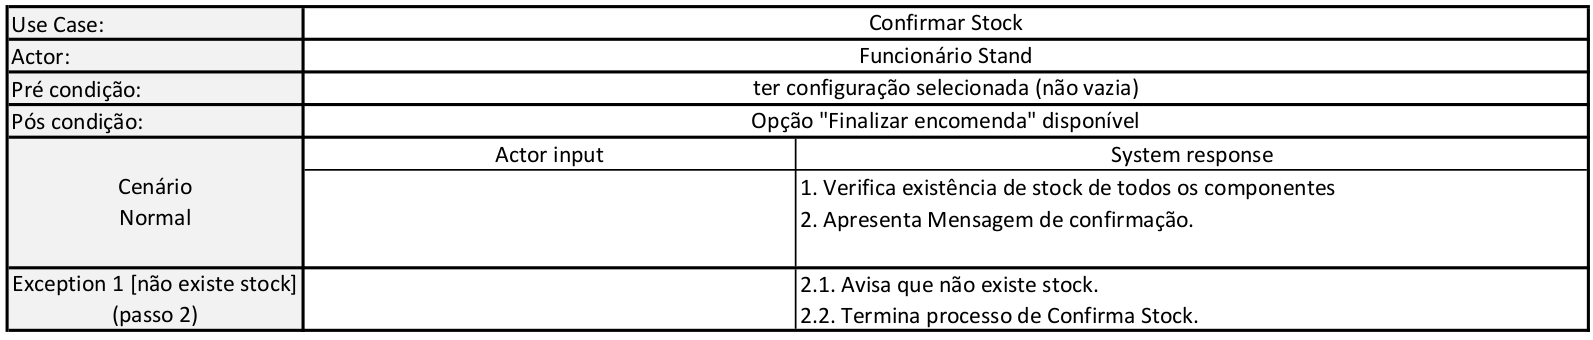
\includegraphics[width=\textwidth]{analise_de_requisitos/img/use_cases/confirmar_stock.png}
    \caption{\textit{Use case}: Confirmar Stock}
    \label{fig:uc_confirmar_stock}
\end{figure}

\begin{figure}[ht]
    \centering
    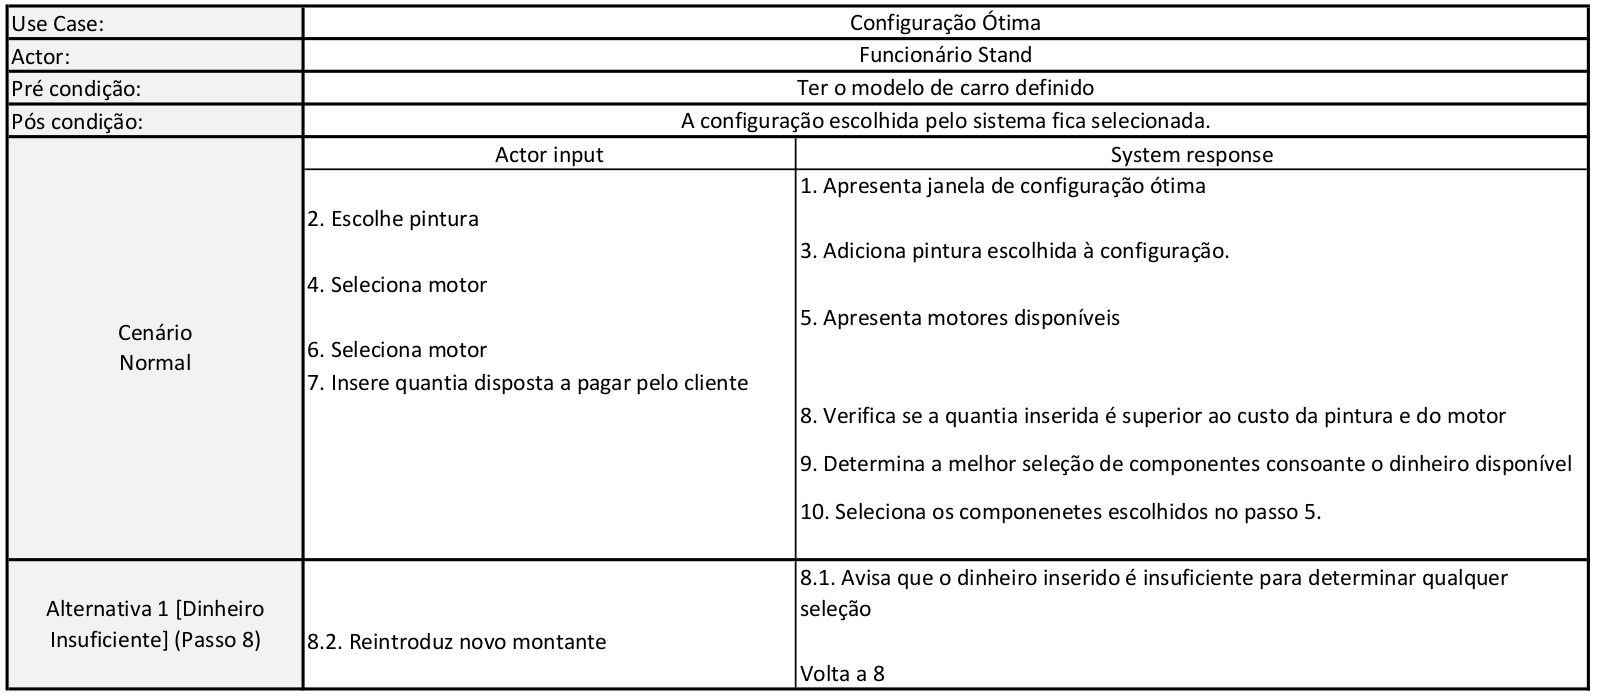
\includegraphics[width=\textwidth]{analise_de_requisitos/img/use_cases/configuracao_otima.png}
    \caption{\textit{Use case}: Configuração Ótima}
    \label{fig:uc_configuracao_otima}
\end{figure}

\begin{figure}[ht]
    \centering
    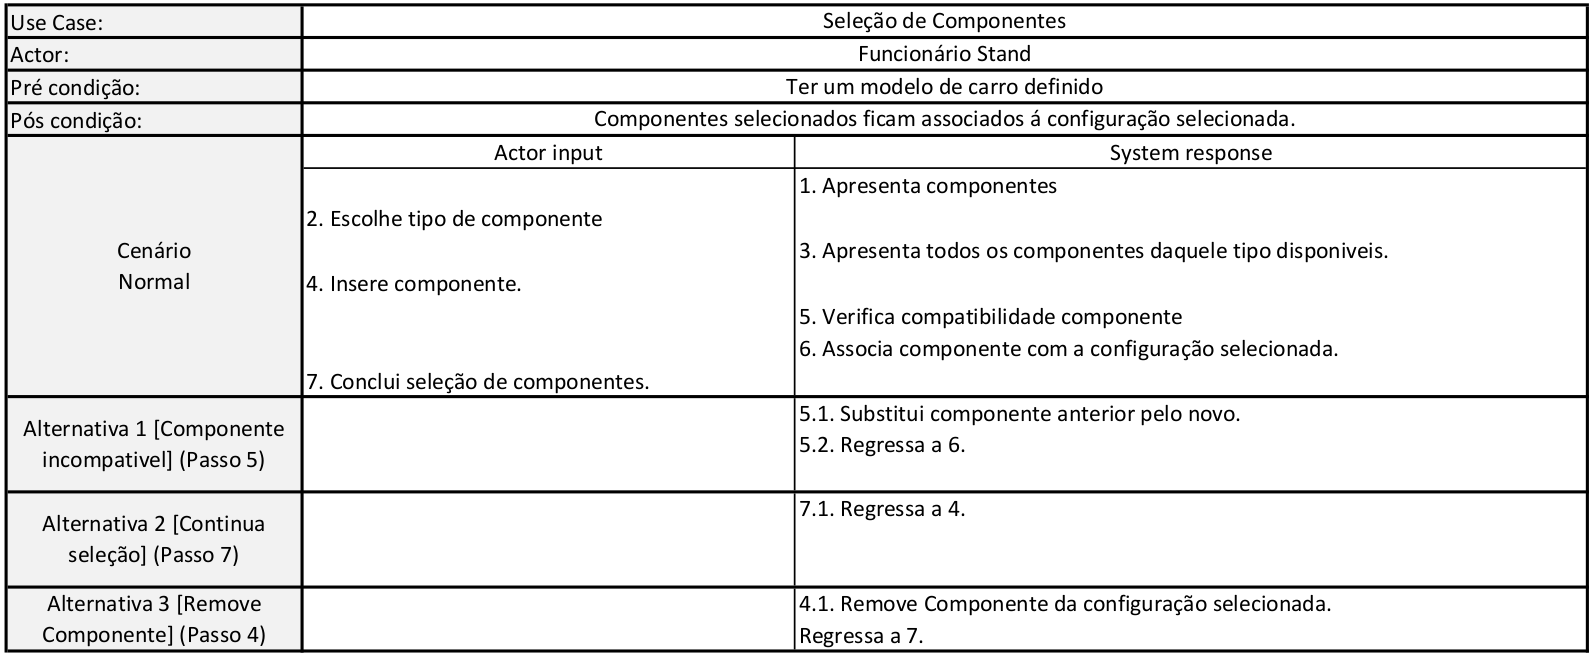
\includegraphics[width=\textwidth]{analise_de_requisitos/img/use_cases/selecao_componentes.png}
    \caption{\textit{Use case}: Seleção de Componentes}
    \label{fig:uc_selecao_componentes}
\end{figure}

\begin{figure}[ht]
    \centering
    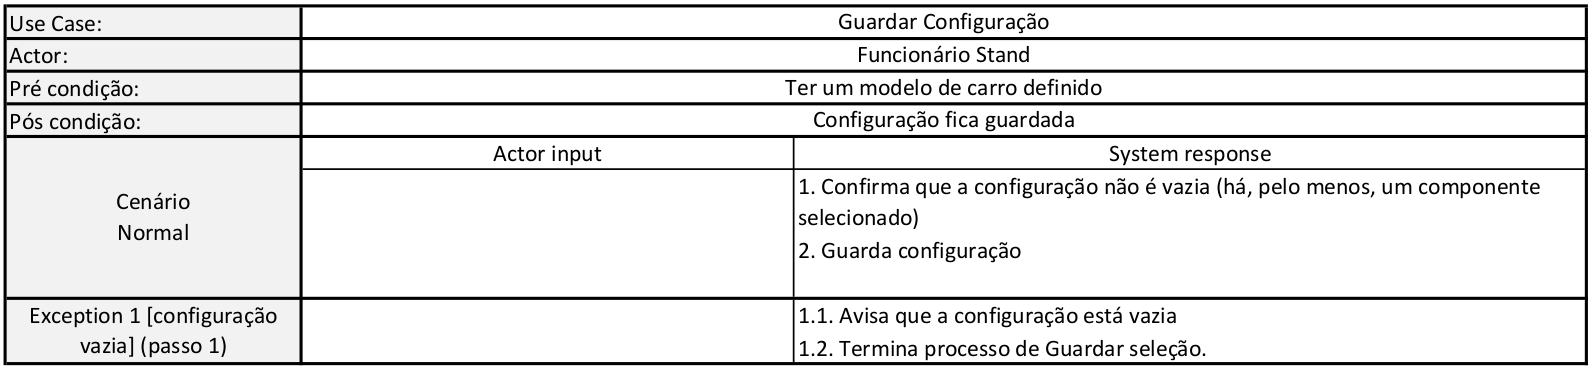
\includegraphics[width=\textwidth]{analise_de_requisitos/img/use_cases/guardar_configuracao.png}
    \caption{\textit{Use case}: Guardar Configuração}
    \label{fig:uc_guardar_configuracao}
\end{figure}

\begin{figure}[ht]
    \centering
    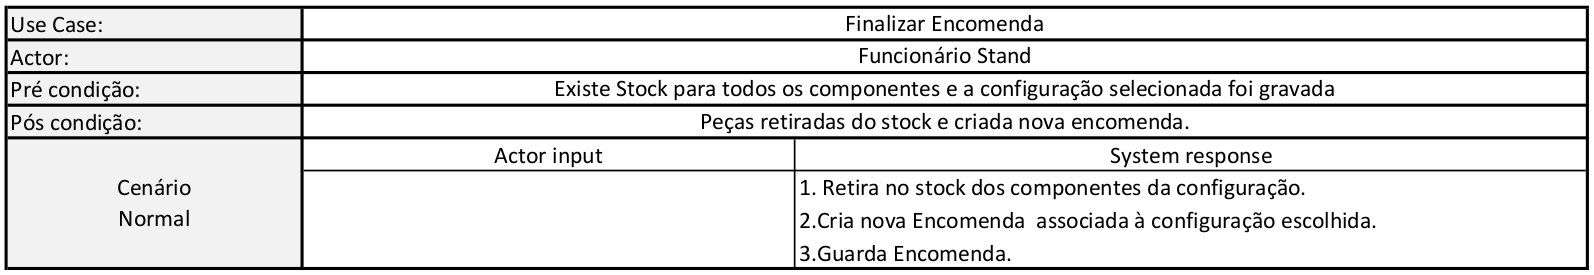
\includegraphics[width=\textwidth]{analise_de_requisitos/img/use_cases/finalizar_encomenda.png}
    \caption{\textit{Use case}: Finalizar Encomenda}
    \label{fig:uc_finalizar_encomenda}
\end{figure}

\begin{figure}[ht]
    \centering
    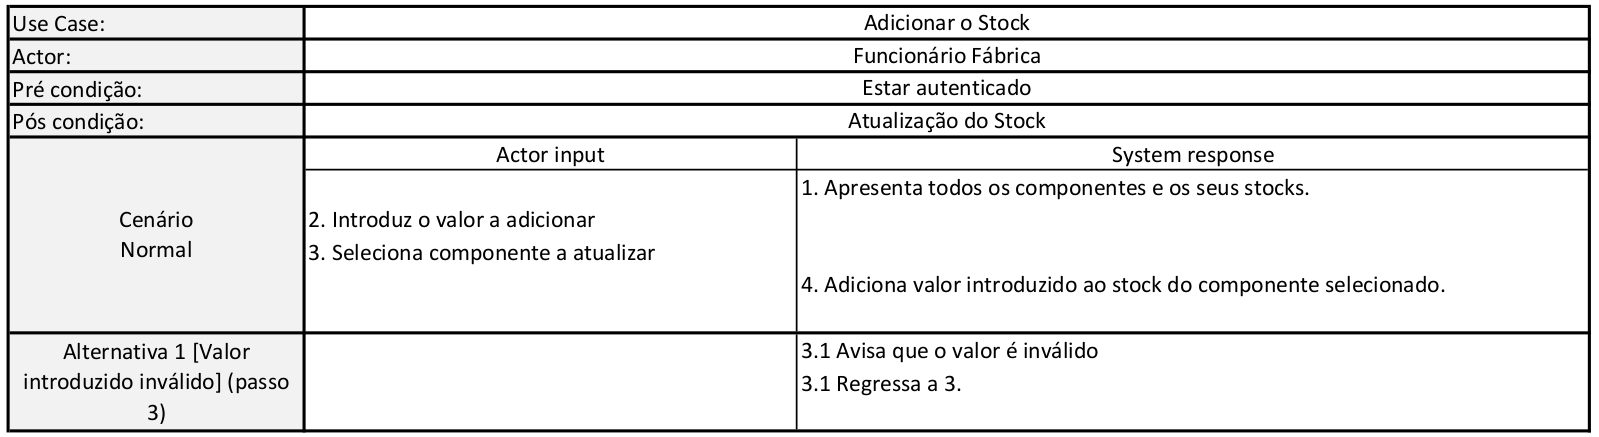
\includegraphics[width=\textwidth]{analise_de_requisitos/img/use_cases/adicionar_stock.png}
    \caption{\textit{Use case}: Adicionar o Stock}
    \label{fig:uc_adicionar_stock}
\end{figure}

\clearpage
    \section{Protótipo de interface gráfica}

Nesta secção encontra-se a nossa proposta de uma interface para todo o sistema. Incluímos também os ficheiros de Netbeans fora do relatório, para possibilitar uma exposição mais direta.

\begin{figure}[h]
    \centering
    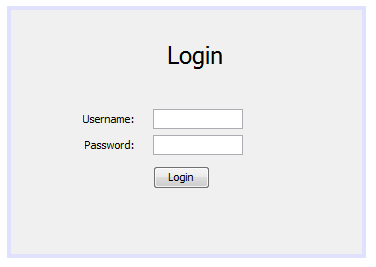
\includegraphics[width=\textwidth]{analise_de_requisitos/img/login.png}
    \caption{Janela de \textit{login}}
\end{figure}

\begin{figure}
    \centering
    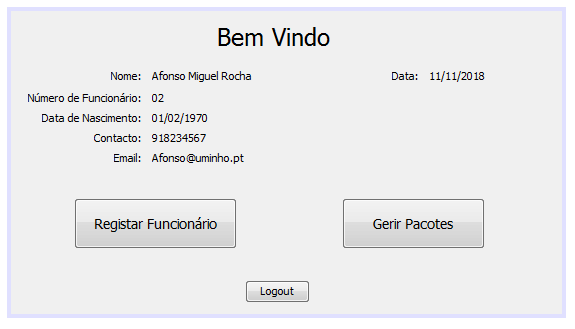
\includegraphics[width=\textwidth]{analise_de_requisitos/img/lobby_admin.png}
    \caption{Lobby do administrador}
\end{figure}

\begin{figure}
    \centering
    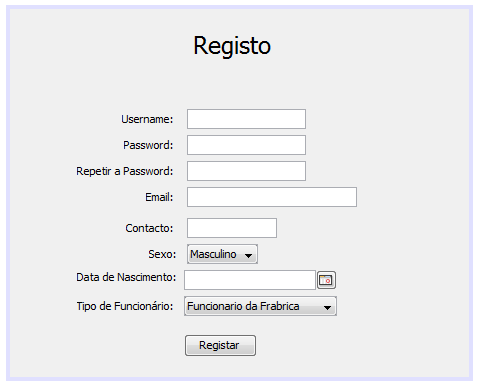
\includegraphics[width=\textwidth]{analise_de_requisitos/img/registo.png}
    \caption{Registo (feito pelo \textit{admin})}
\end{figure}

\begin{figure}
    \centering
    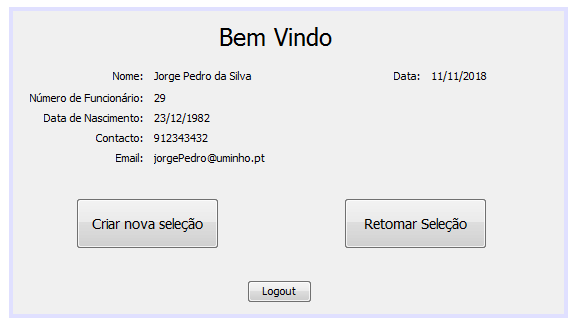
\includegraphics[width=\textwidth]{analise_de_requisitos/img/lobby_funcionario.png}
    \caption{Lobby do funcionário do Stand}
\end{figure}

\begin{figure}
    \centering
    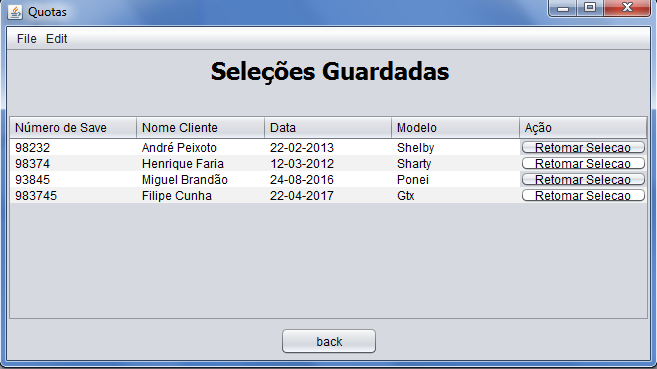
\includegraphics[width=\textwidth]{analise_de_requisitos/img/configs_guardadas.png}
    \caption{Janela das configurações guardadas}
\end{figure}

\begin{figure}
    \centering
    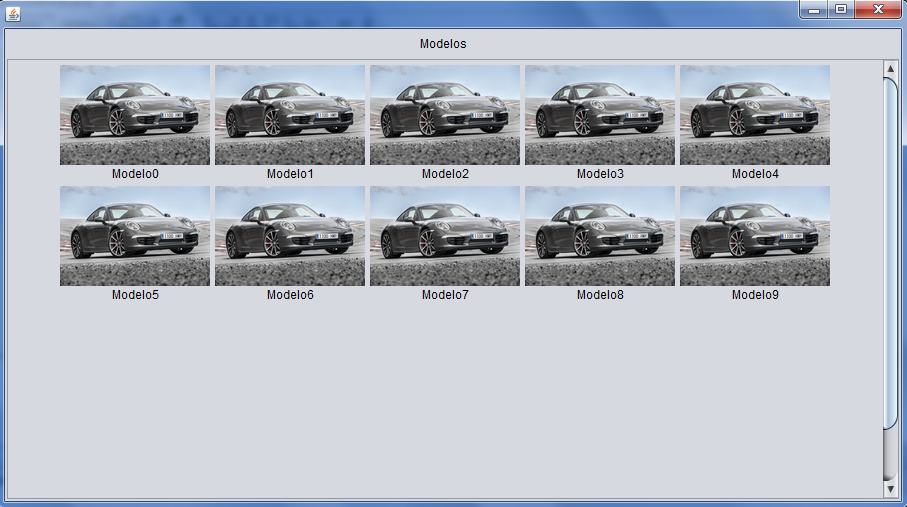
\includegraphics[width=\textwidth]{analise_de_requisitos/img/config_escolher_modelo.png}
    \caption{Primeira janela do processo de configuração (escolher modelo)}
\end{figure}

\begin{figure}
    \centering
    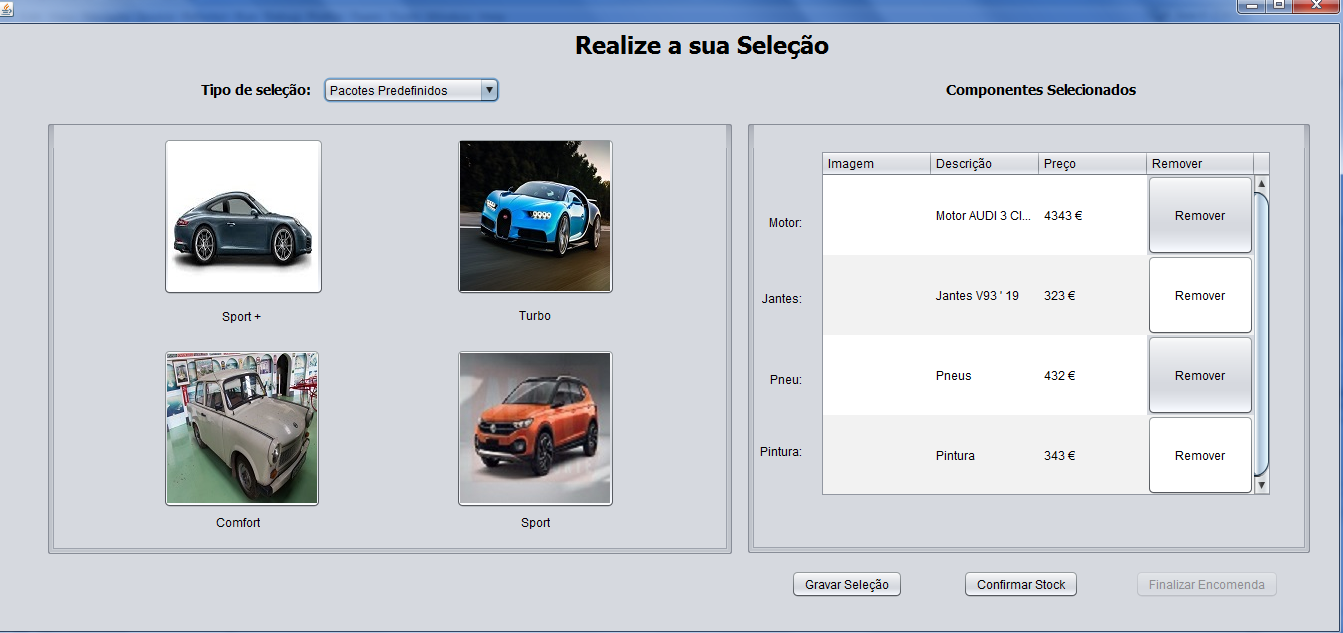
\includegraphics[width=\textwidth]{analise_de_requisitos/img/config_guardar_finalizar.png}
    \caption{Segunda janela do processo de configuração (escolher o tipo de seleção/gravar/confirmar/finalizar encomenda)}
\end{figure}

\begin{figure}
    \centering
    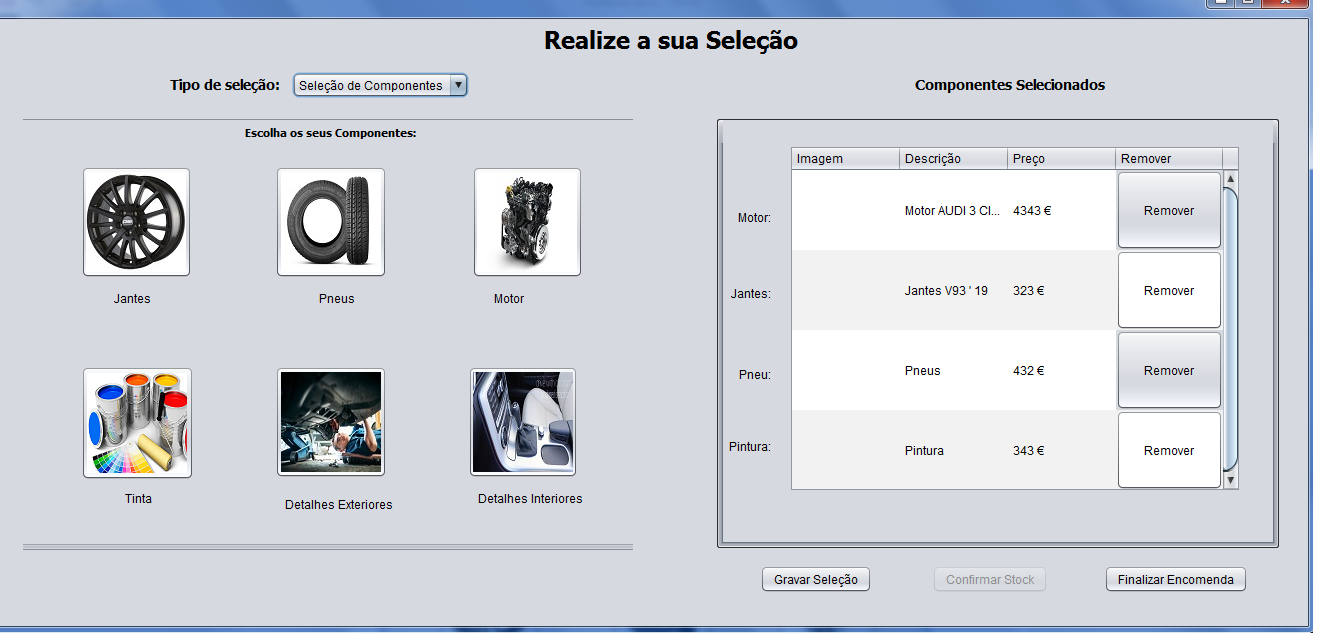
\includegraphics[width=\textwidth]{analise_de_requisitos/img/config_selecao_componentes_manual_1.png}
    \caption{Seleção de componentes manual (1/2)}
\end{figure}

\begin{figure}
    \centering
    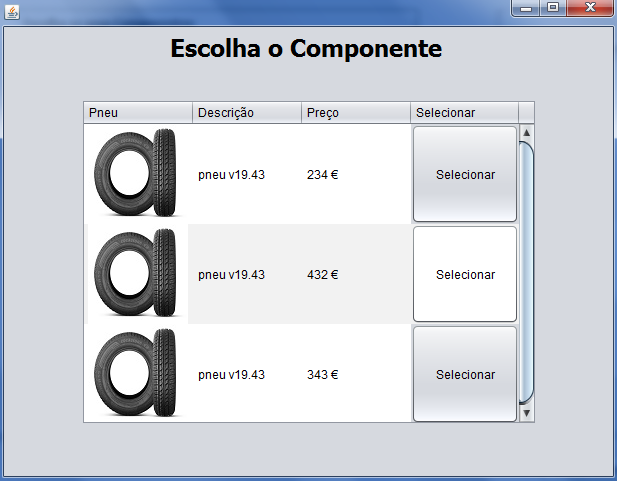
\includegraphics[width=\textwidth]{analise_de_requisitos/img/config_selecao_componentes_manual_2.png}
    \caption{Seleção de componentes manual (2/2)}
\end{figure}

\begin{figure}
    \centering
    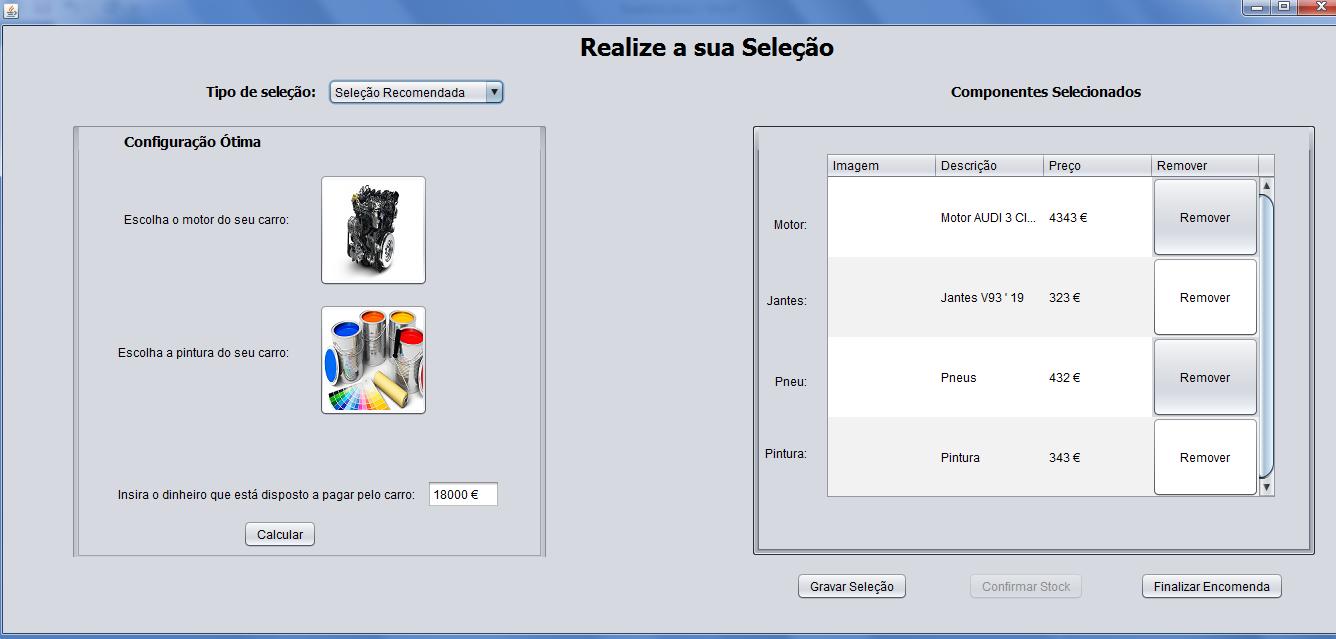
\includegraphics[width=\textwidth]{analise_de_requisitos/img/config_otima.png}
    \caption{Configuração ótima automática}
\end{figure}

\begin{figure}
    \centering
    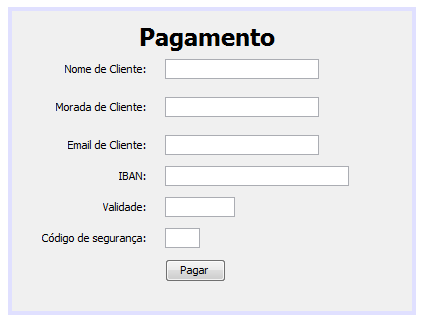
\includegraphics[width=\textwidth]{analise_de_requisitos/img/config_finalizar.png}
    \caption{Finalizar configuração}
\end{figure}

\begin{figure}
    \centering
    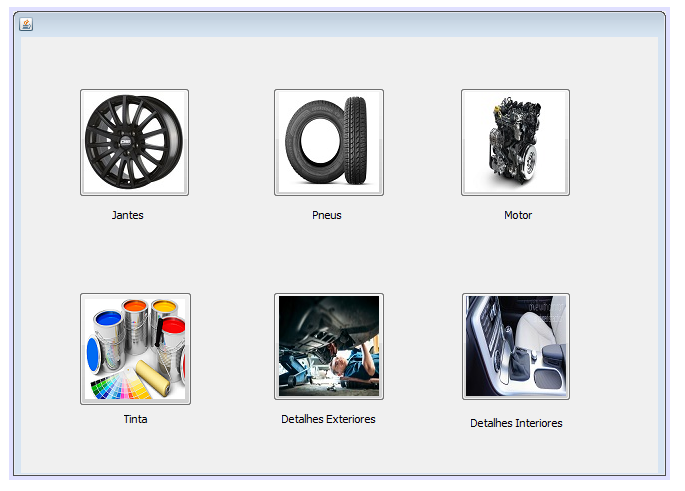
\includegraphics[width=\textwidth]{analise_de_requisitos/img/lobby_fabrica.png}
    \caption{Lobby do funcionário de fábrica (escolher o que quer atualizar)}
\end{figure}

\begin{figure}
    \centering
    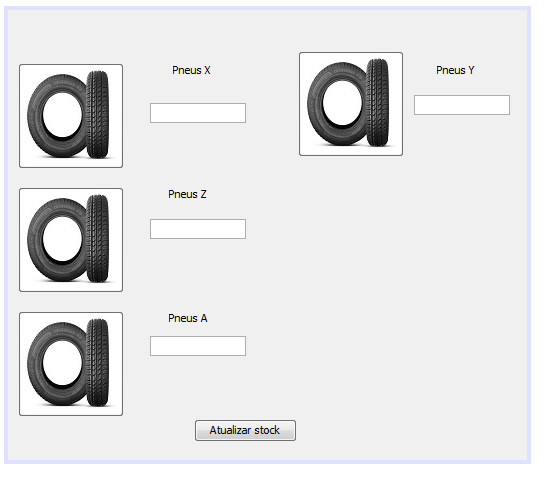
\includegraphics[width=\textwidth]{analise_de_requisitos/img/atualizar_stock_pneus.png}
    \caption{Atualizar stock de pneus}
\end{figure}

\begin{figure}
    \centering
    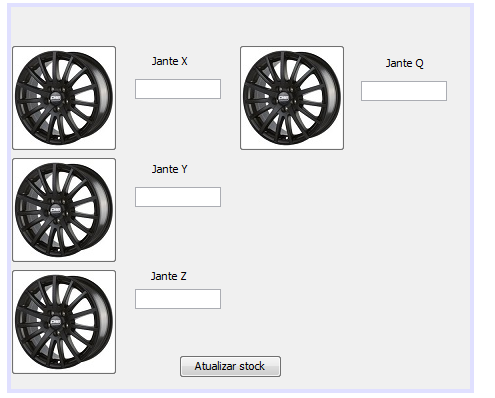
\includegraphics[width=\textwidth]{analise_de_requisitos/img/atualizar_stock_jantes.png}
    \caption{Atualizar stock de jantes}
\end{figure}

\begin{figure}
    \centering
    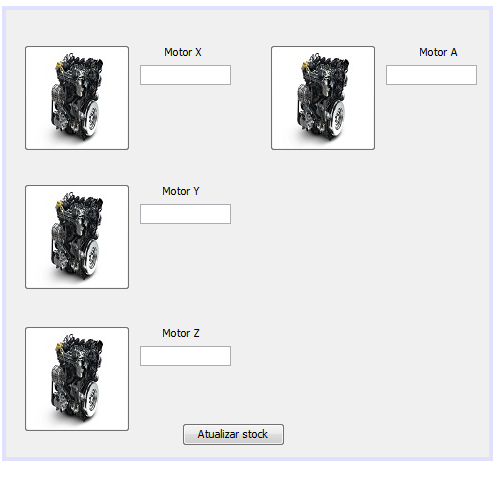
\includegraphics[width=\textwidth]{analise_de_requisitos/img/atualizar_stock_motores.png}
    \caption{Atualizar stock de motores}
\end{figure}

\begin{figure}
    \centering
    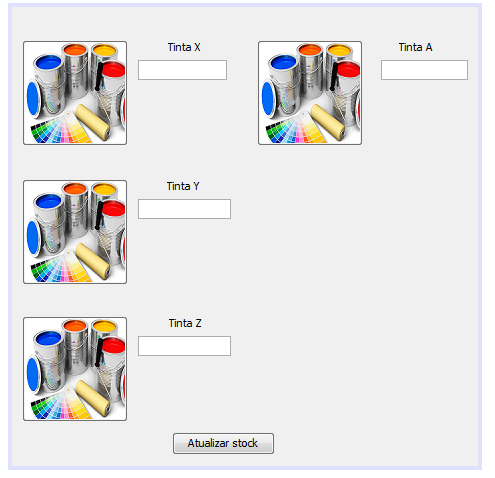
\includegraphics[width=\textwidth]{analise_de_requisitos/img/atualizar_stock_tintas.png}
    \caption{Atualizar stock de tintas}
\end{figure}



\clearpage
    \section{Diagrama de estados}

Nesta secção, apresentamos o diagrama de estado do nosso sistema (figura \ref{fig:diagrama_de_estado}).

\begin{figure}[h]
    \centering
    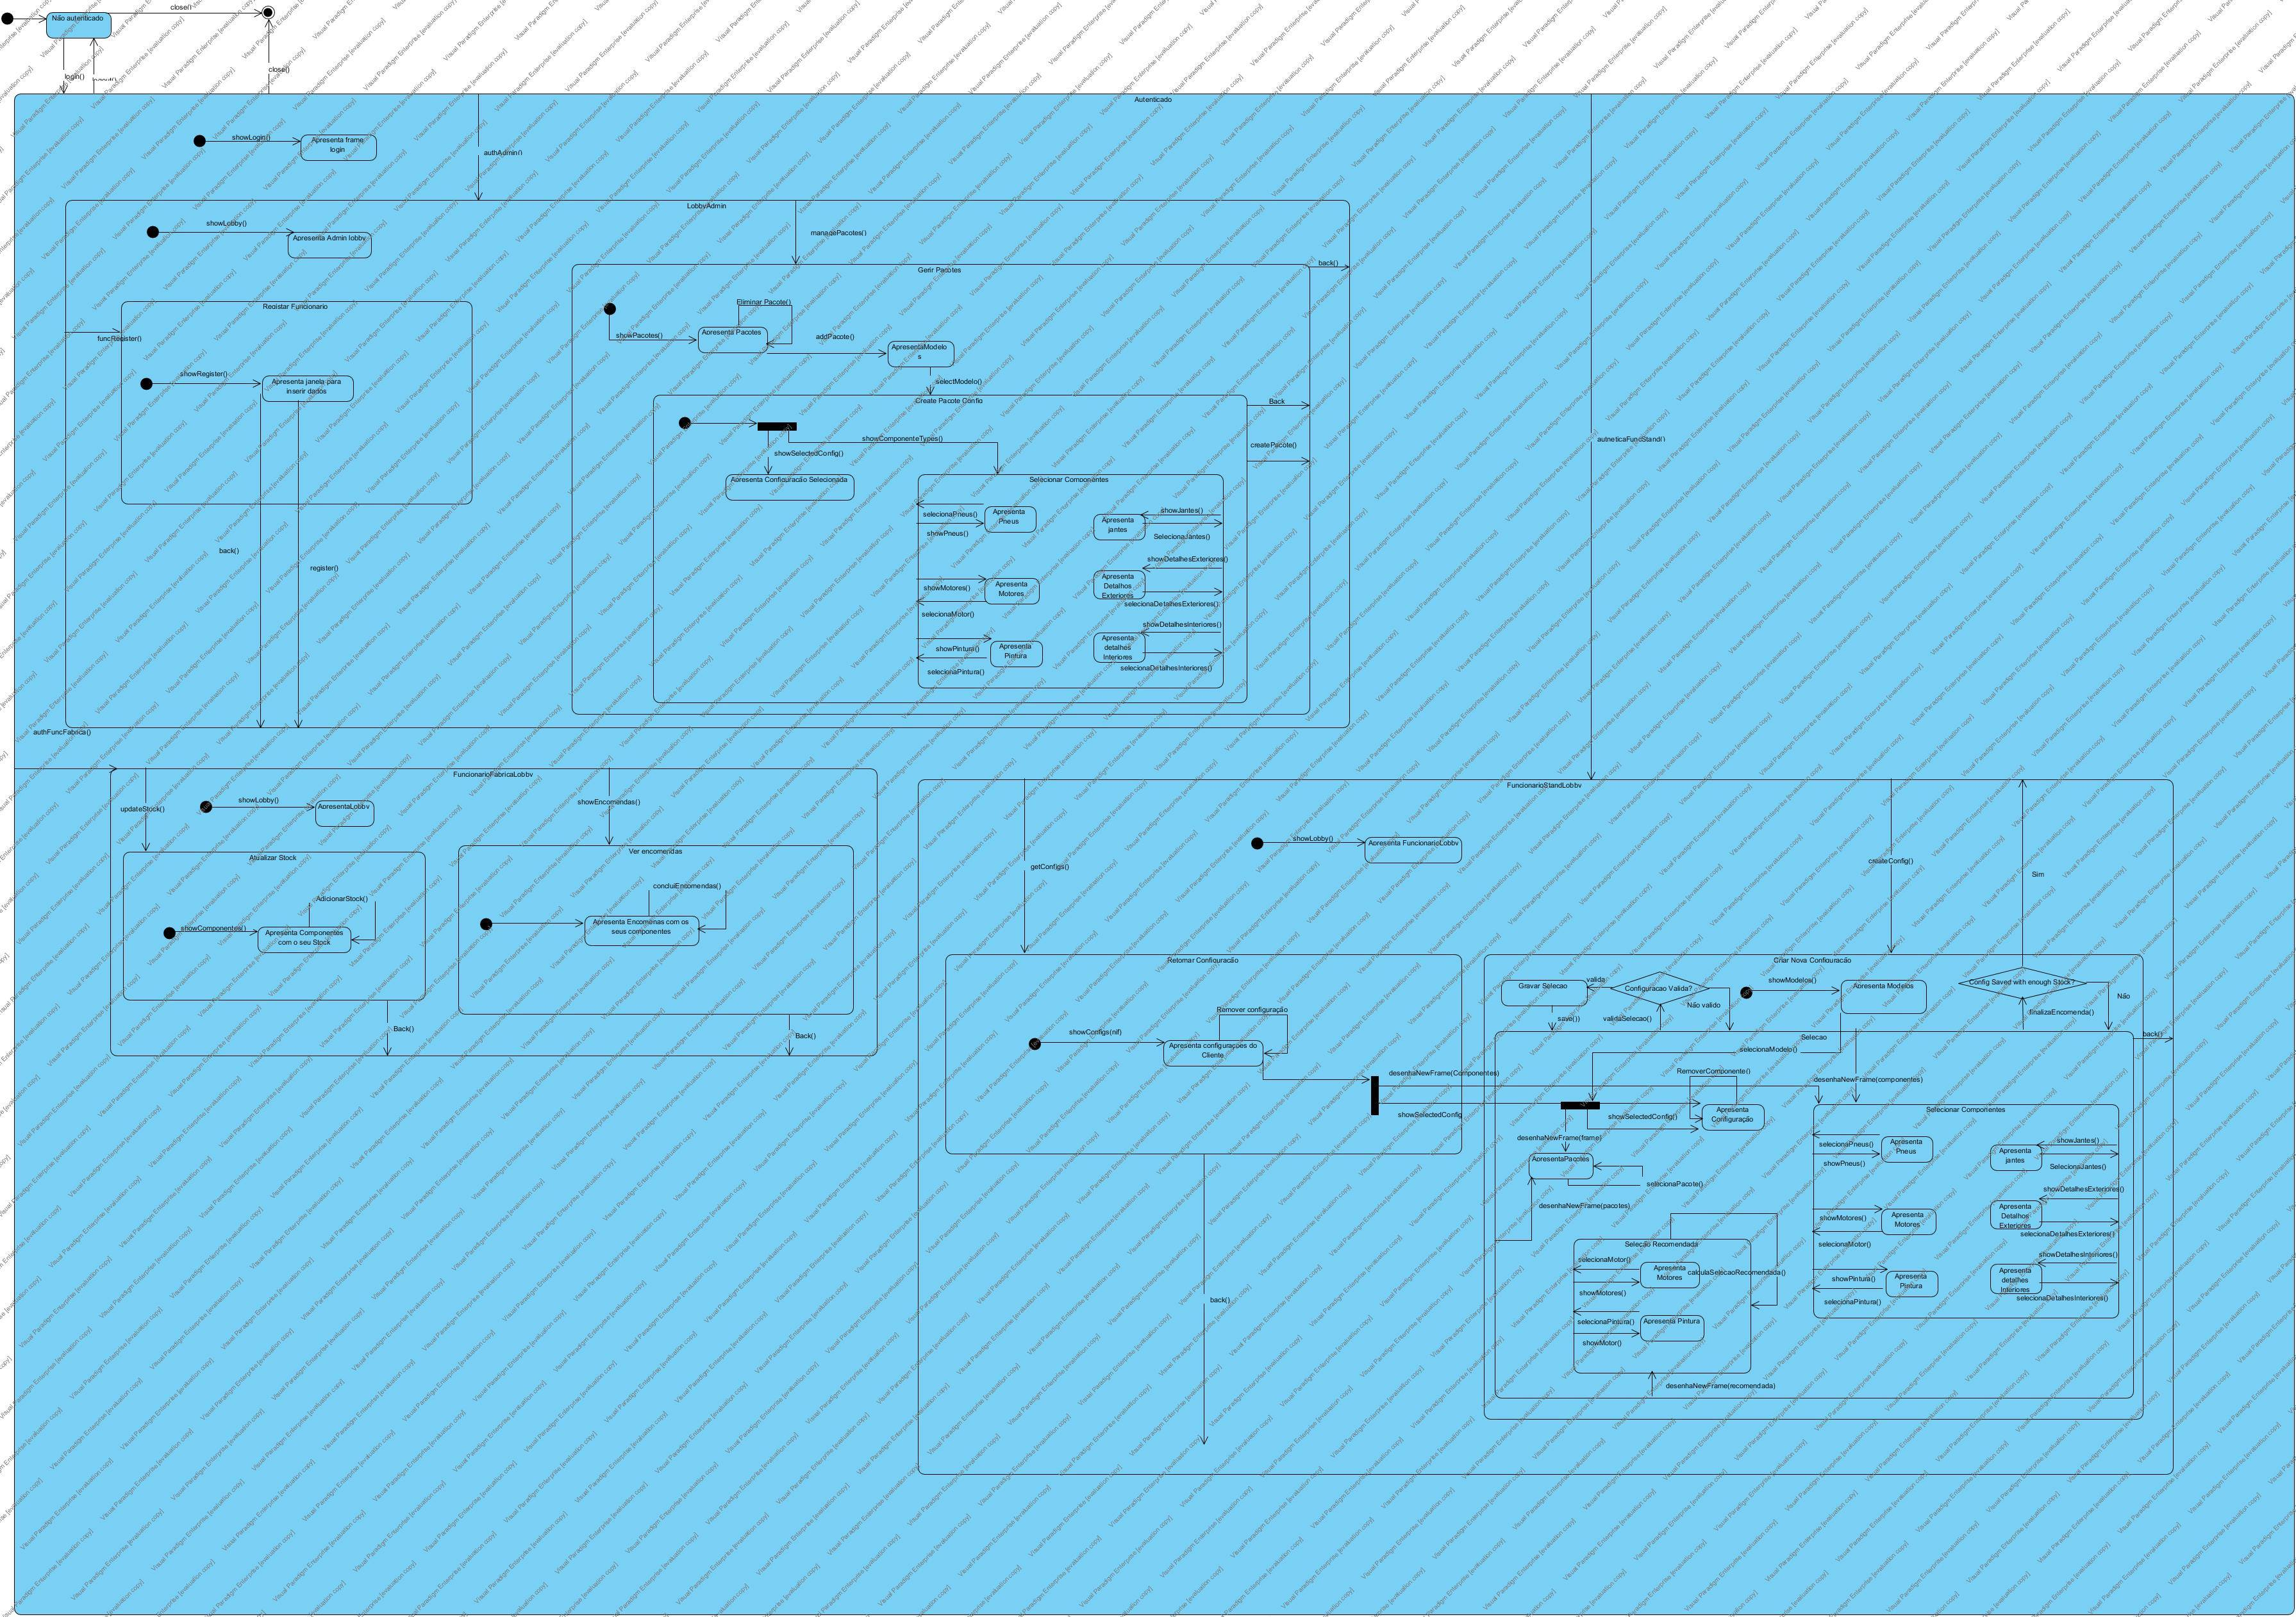
\includegraphics[width=\textwidth]{analise_de_requisitos/49461754_398655354223097_8464874533138989056_n.jpg}
    \caption{Diagrama de estado}
    \label{fig:diagrama_de_estado}
\end{figure}


Neste diagrama, admitimos que existe um superestado chamado “autenticado”, que surge quando se efetua o \textit{login}. Este estado direciona o utilizador para diferentes subestados, dependendo da sua função no sistema. Se o utilizador for um funcionário de fábrica, este tem acesso ao métodos representados no lado esquerdo do modelo acima, que correspondem à atualização do stock (jantes, motores, pintura e pneus). Se o utilizador for um administrador, só tem acesso aos métodos que lhe permitem registar funcionários e criar/eliminar pacotes do sistema. Por último, todos os funcionários de stand têm acesso às funcionalidades faladas já nas secções anteriores, que estão representadas no lado direito do superestado do diagrama (fig. \ref{fig:diagrama_de_estado}).


\clearpage
    \section{Diagramas de sequência}

Nesta secção, encontram-se os diagramas de sequência dos vários use cases referidos na figura \ref{fig:diagrama_de_use_cases}. Para cada use case existem três diagramas: os D1, os mais básicos, que apenas registam a interação entre o utilizador e o sistema; os D2, que especificam as interações representadas nos D1 mas divididas entre as camadas lógicas do programa e os D3, que especificam as interações dos D3 mas utilizando métodos.

Abaixo estão os diagramas do referentes use cases:

\subsection{Autenticação}

\begin{figure}[H]
    \centering
    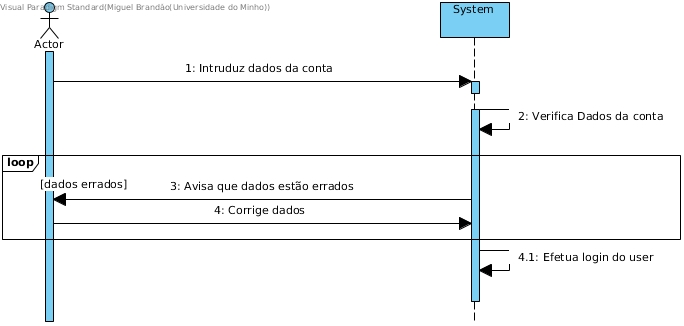
\includegraphics[width=\textwidth]{diagramas_de_sequencia/imgs/UserSystemUC1.jpg}
    \caption{D1}
\end{figure}
\begin{figure}[H]
    \centering
    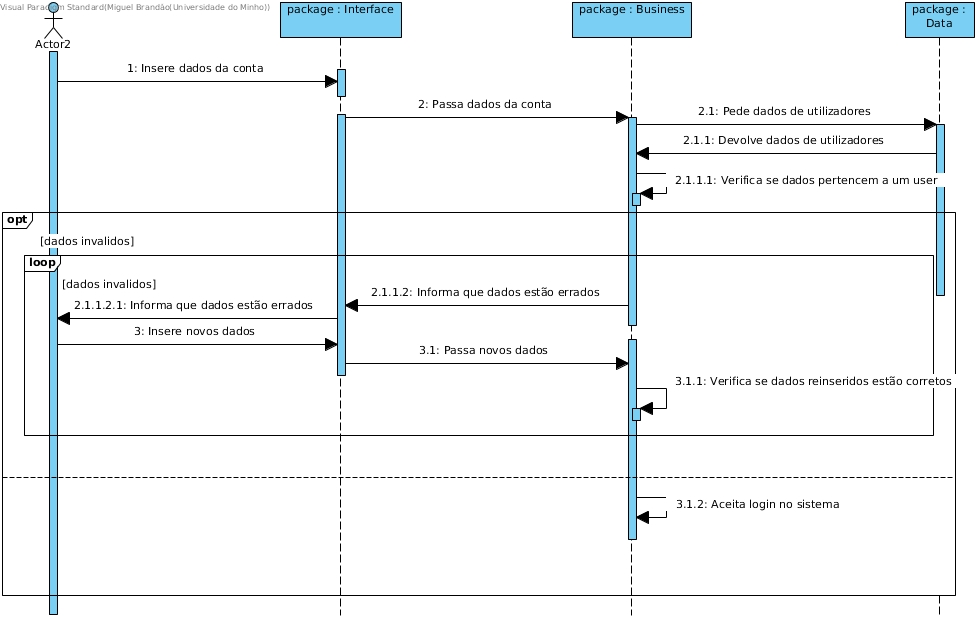
\includegraphics[width=\textwidth]{diagramas_de_sequencia/imgs/UserSystemUC1D2.jpg}
    \caption{D2}
\end{figure}
\begin{figure}[H]
    \centering
    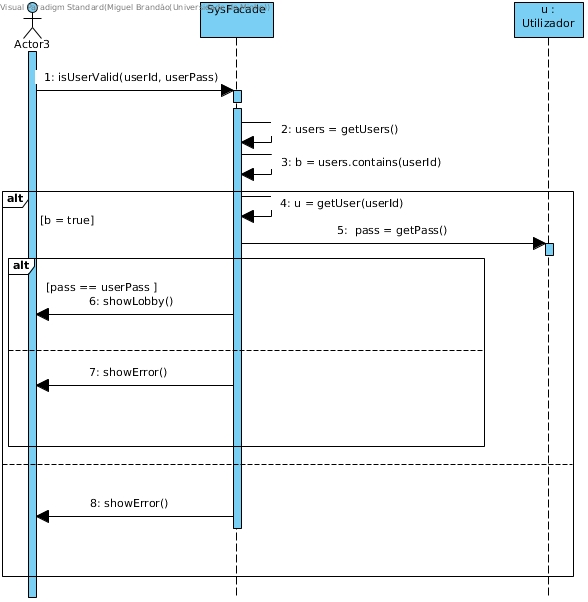
\includegraphics[width=\textwidth]{diagramas_de_sequencia/imgs/UserSystemUC1D3.jpg}
    \caption{D3}
\end{figure}

\subsection{Logout}

\begin{figure}[H]
    \centering
    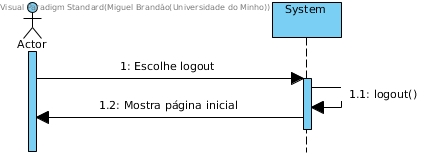
\includegraphics[width=\textwidth]{diagramas_de_sequencia/imgs/UserSystemUC2D1.jpg}
    \caption{D1}
\end{figure}
\begin{figure}[H]
    \centering
    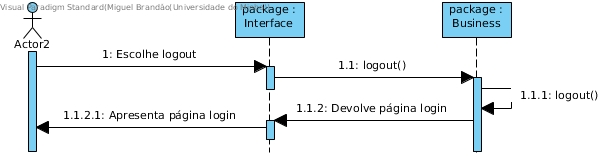
\includegraphics[width=\textwidth]{diagramas_de_sequencia/imgs/UserSystemUC2D2.jpg}
    \caption{D2}
\end{figure}
\begin{figure}[H]
    \centering
    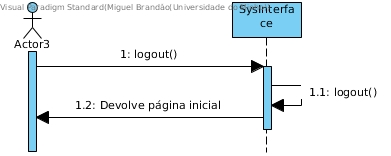
\includegraphics[width=\textwidth]{diagramas_de_sequencia/imgs/UserSystemUC2D3.jpg}
    \caption{D3}
\end{figure}

\subsection{Registo}

\begin{figure}[H]
    \centering
    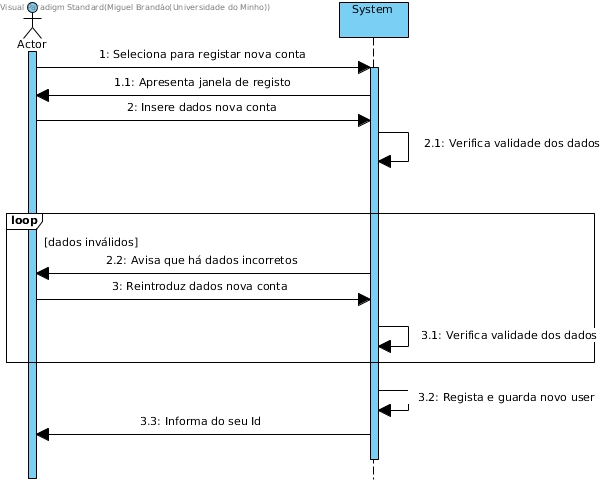
\includegraphics[width=\textwidth]{diagramas_de_sequencia/imgs/UserSystemUC3D1.jpg}
    \caption{D1}
\end{figure}
\begin{figure}[H]
    \centering
    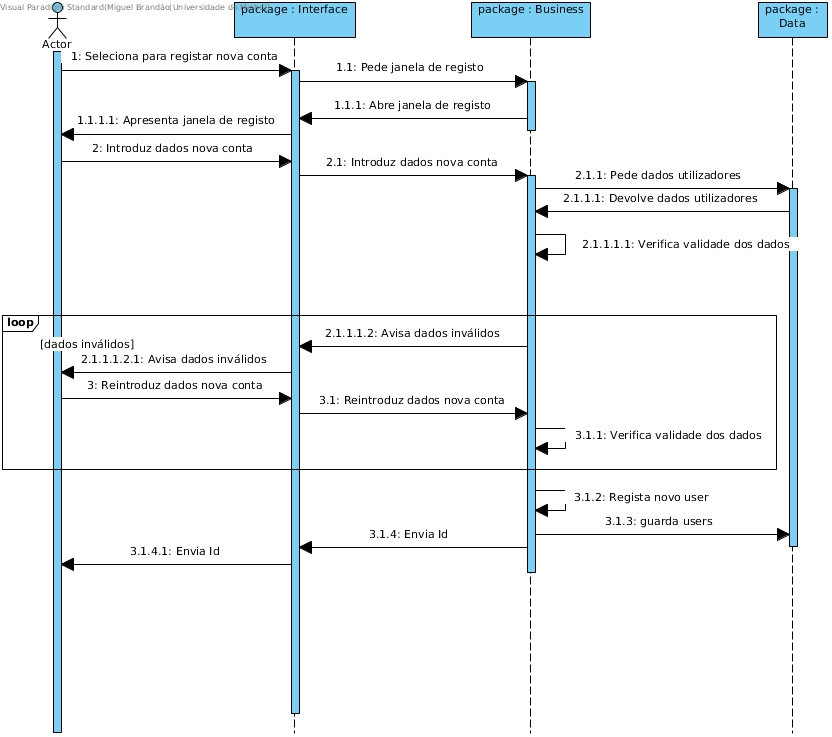
\includegraphics[width=\textwidth]{diagramas_de_sequencia/imgs/UserSystemUC3D2.jpg}
    \caption{D2}
\end{figure}
\begin{figure}[H]
    \centering
    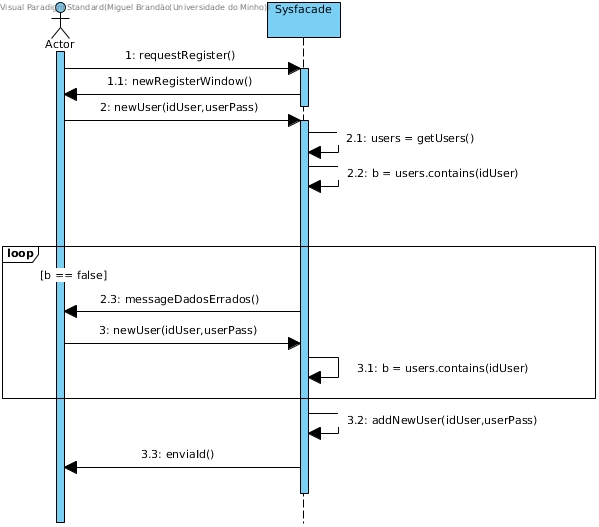
\includegraphics[width=\textwidth]{diagramas_de_sequencia/imgs/UserSystemUC3D3.jpg}
    \caption{D3}
\end{figure}

\subsection{Criar Pacote}

\begin{figure}[H]
    \centering
    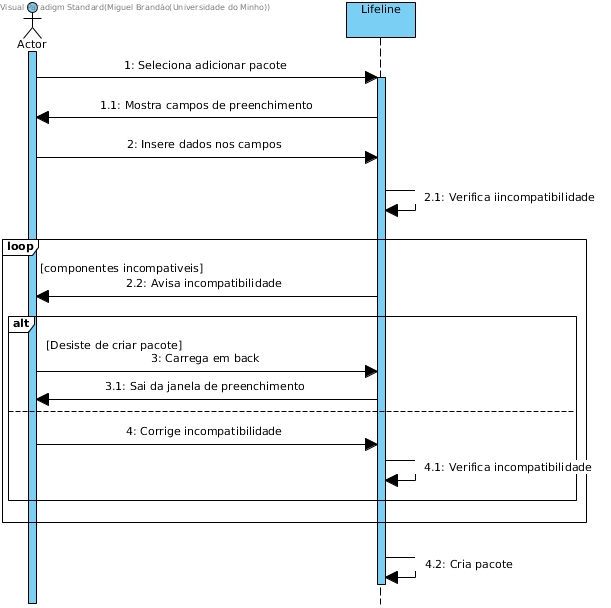
\includegraphics[width=\textwidth]{diagramas_de_sequencia/imgs/UserSystemUC4D1.jpg}
    \caption{D1}
\end{figure}
\begin{figure}[H]
    \centering
    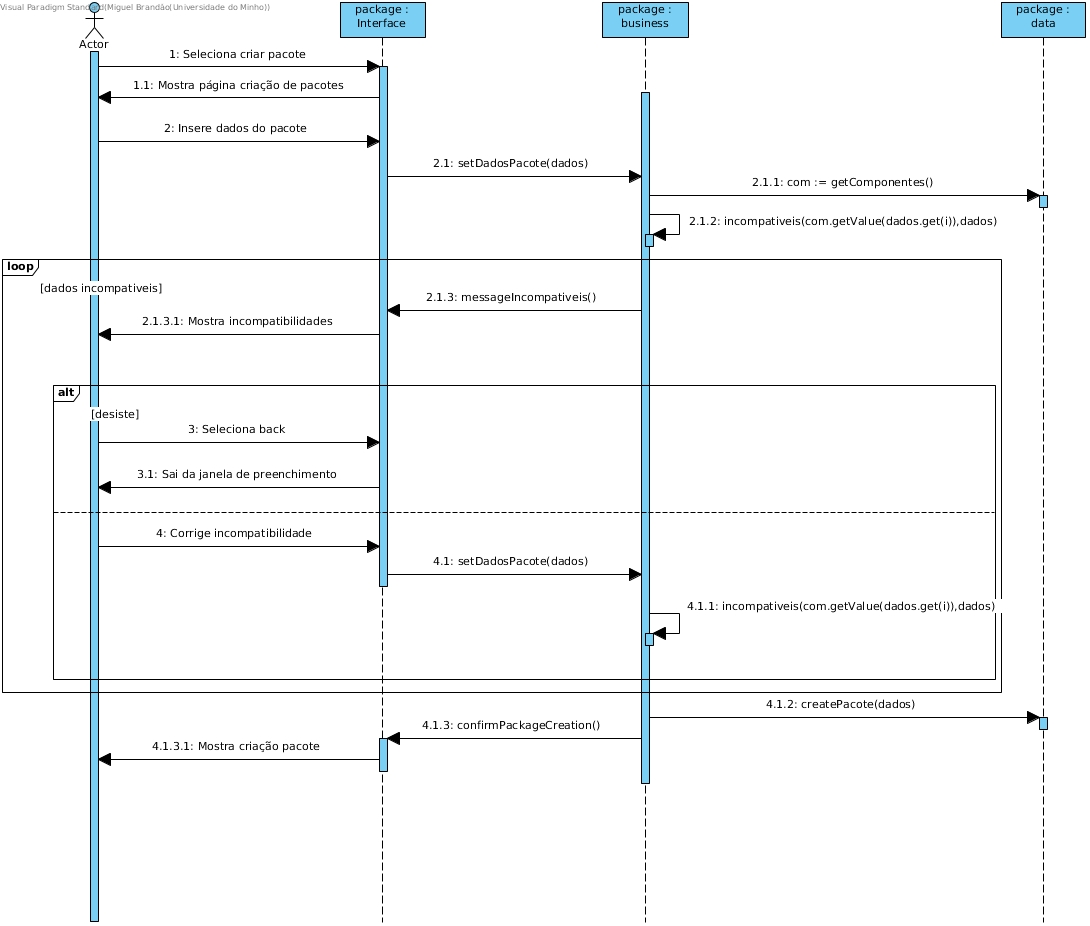
\includegraphics[width=\textwidth]{diagramas_de_sequencia/imgs/UserSystemUC4D2.jpg}
    \caption{D2}
\end{figure}
\begin{figure}[H]
    \centering
    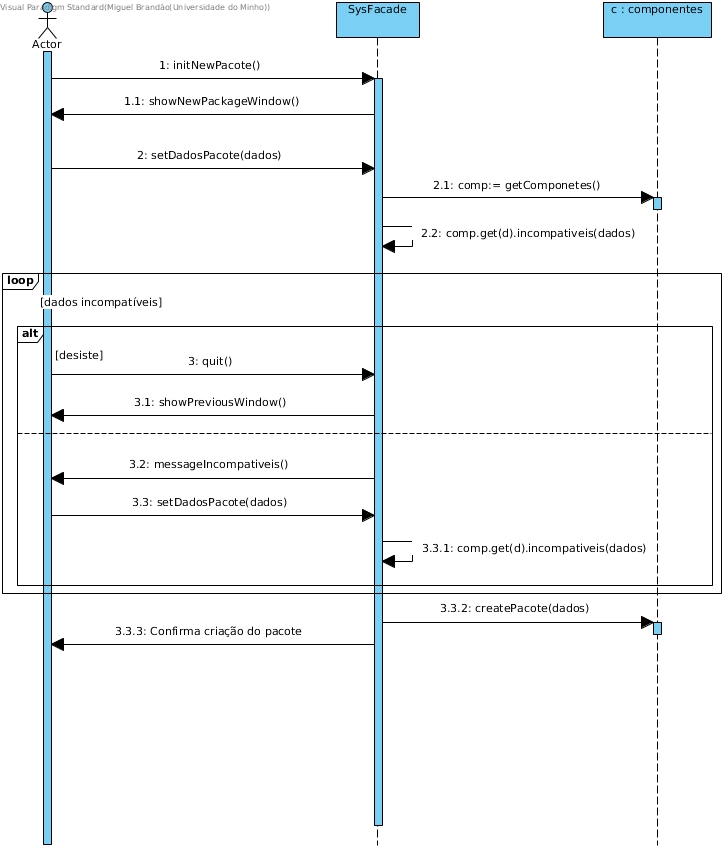
\includegraphics[width=\textwidth]{diagramas_de_sequencia/imgs/UserSystemUC4D3.jpg}
    \caption{D3}
\end{figure}

\subsection{Eliminar Pacote}

\begin{figure}[H]
    \centering
    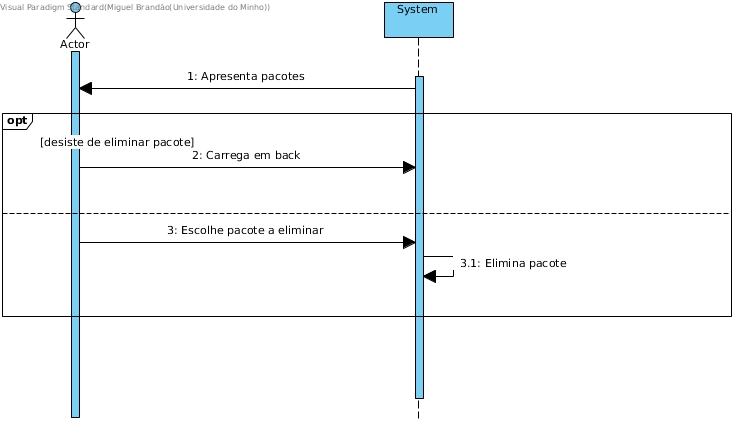
\includegraphics[width=\textwidth]{diagramas_de_sequencia/imgs/UserSystemUC5D1.jpg}
    \caption{D1}
\end{figure}
\begin{figure}[H]
    \centering
    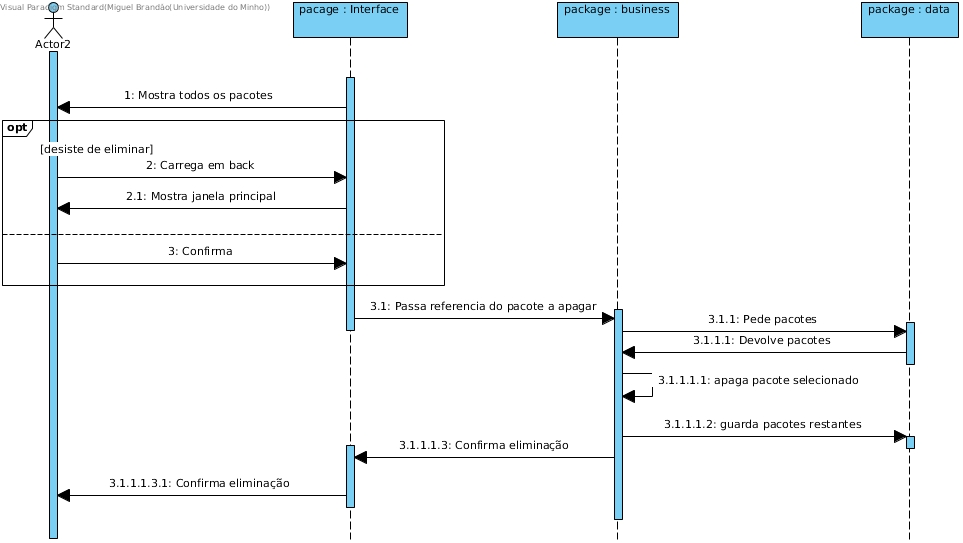
\includegraphics[width=\textwidth]{diagramas_de_sequencia/imgs/UserSystemUC5D2.jpg}
    \caption{D2}
\end{figure}
\begin{figure}[H]
    \centering
    \includegraphics[width=\textwidth]{diagramas_de_sequencia/imgs/UserSystemUC5D3.jpg}
    \caption{D3}
\end{figure}

\subsection{Retomar Configuração}

\begin{figure}[H]
    \centering
    \includegraphics[width=\textwidth]{diagramas_de_sequencia/imgs/UserSystemUC6D1.jpg}
    \caption{D1}
\end{figure}
\begin{figure}[H]
    \centering
    \includegraphics[width=\textwidth]{diagramas_de_sequencia/imgs/UserSystemUC6D2.jpg}
    \caption{D2}
\end{figure}
\begin{figure}[H]
    \centering
    \includegraphics[width=\textwidth]{diagramas_de_sequencia/imgs/UserSystemUC6D3.jpg}
    \caption{D3}
\end{figure}
\subsection{Apagar Configuração}

\begin{figure}[H]
    \centering
    \includegraphics[width=\textwidth]{diagramas_de_sequencia/imgs/UC7D1.jpg}
    \caption{D1}
\end{figure}
\begin{figure}[H]
    \centering
    \includegraphics[width=\textwidth]{diagramas_de_sequencia/imgs/UC7D2.jpg}
    \caption{D2}
\end{figure}
\begin{figure}[H]
    \centering
    \includegraphics[width=\textwidth]{diagramas_de_sequencia/imgs/UC7D3.jpg}
    \caption{D3}
\end{figure}
\begin{comment}

\subsection{Seleção de Configuração}

\begin{figure}[H]
    \centering
    \includegraphics[width=\textwidth]{diagramas_de_sequencia/imgs/
    \caption{D1}
\end{figure}
\begin{figure}[H]
    \centering
    \includegraphics[width=\textwidth]{diagramas_de_sequencia/imgs/
    \caption{D2}
\end{figure}
\begin{figure}[H]
    \centering
    \includegraphics[width=\textwidth]{diagramas_de_sequencia/imgs/
    \caption{D3}
\end{figure}
\end{comment}
\subsection{Seleção do Modelo de Carro}

\begin{figure}[H]
    \centering
    \includegraphics[width=\textwidth]{diagramas_de_sequencia/imgs/UserSystemUC8D1.jpg}
    \caption{D1}
\end{figure}
\begin{figure}[H]
    \centering
    \includegraphics[width=\textwidth]{diagramas_de_sequencia/imgs/UserSystemUC8D2.jpg}
    \caption{D2}
\end{figure}
\begin{figure}[H]
    \centering
    \includegraphics[width=\textwidth]{diagramas_de_sequencia/imgs/UserSystemUC8D3.jpg}
    \caption{D3}
\end{figure}

\subsection{Seleção do Pacote}

\begin{figure}[H]
    \centering
    \includegraphics[width=\textwidth]{diagramas_de_sequencia/imgs/UserSystemUC9D1.jpg}
    \caption{D1}
\end{figure}
\begin{figure}[H]
    \centering
    \includegraphics[width=\textwidth]{diagramas_de_sequencia/imgs/UserSystemUC9D2.jpg}
    \caption{D2}
\end{figure}
\begin{figure}[H]
    \centering
    \includegraphics[width=\textwidth]{diagramas_de_sequencia/imgs/UserSystemUC9D3.jpg}
    \caption{D3}
\end{figure}
\begin{comment}

\subsection{Confirmar stock}

\begin{figure}[H]
    \centering
    \includegraphics[width=\textwidth]{diagramas_de_sequencia/imgs/
    \caption{D1}
\end{figure}
\begin{figure}[H]
    \centering
    \includegraphics[width=\textwidth]{diagramas_de_sequencia/imgs/
    \caption{D2}
\end{figure}
\begin{figure}[H]
    \centering
    \includegraphics[width=\textwidth]{diagramas_de_sequencia/imgs/
    \caption{D3}
\end{figure}
\end{comment}

\subsection{Configuração Ótima}

\begin{figure}[H]
    \centering
    \includegraphics[width=\textwidth]{diagramas_de_sequencia/imgs/UserSystemUC10D1.jpg}
    \caption{D1}
\end{figure}
\begin{figure}[H]
    \centering
    \includegraphics[width=\textwidth]{diagramas_de_sequencia/imgs/UserSystemUC10D2.jpg}
    \caption{D2}
\end{figure}
\begin{figure}[H]
    \centering
    \includegraphics[width=\textwidth]{diagramas_de_sequencia/imgs/UserSystemUC10D3.jpg}
    \caption{D3}
\end{figure}

\subsection{Seleção de Componentes}

\begin{figure}[H]
    \centering
    \includegraphics[width=\textwidth]{diagramas_de_sequencia/imgs/UserSystemUC11D1.jpg}
    \caption{D1}
\end{figure}
\begin{figure}[H]
    \centering
    \includegraphics[width=\textwidth]{diagramas_de_sequencia/imgs/UserSystemUC11D2.jpg}
    \caption{D2}
\end{figure}
\begin{figure}[H]
    \centering
    \includegraphics[width=\textwidth]{diagramas_de_sequencia/imgs/UserSystemUC11D3.jpg}
    \caption{D3}
\end{figure}
\begin{comment}

\subsection{Guardar Configuração}

\begin{figure}[H]
    \centering
    \includegraphics[width=\textwidth]{diagramas_de_sequencia/imgs/
    \caption{D1}
\end{figure}
\begin{figure}[H]
    \centering
    \includegraphics[width=\textwidth]{diagramas_de_sequencia/imgs/
    \caption{D2}
\end{figure}
\begin{figure}[H]
    \centering
    \includegraphics[width=\textwidth]{diagramas_de_sequencia/imgs/
    \caption{D3}
\end{figure}

\subsection{Finalizar Encomenda}

\begin{figure}[H]
    \centering
    \includegraphics[width=\textwidth]{diagramas_de_sequencia/imgs/
    \caption{D1}
\end{figure}
\begin{figure}[H]
    \centering
    \includegraphics[width=\textwidth]{diagramas_de_sequencia/imgs/
    \caption{D2}
\end{figure}
\begin{figure}[H]
    \centering
    \includegraphics[width=\textwidth]{diagramas_de_sequencia/imgs/
    \caption{D3}
\end{figure}

\subsection{Adicionar o Stock}

\begin{figure}[H]
    \centering
    \includegraphics[width=\textwidth]{diagramas_de_sequencia/imgs/
    \caption{D1}
\end{figure}
\begin{figure}[H]
    \centering
    \includegraphics[width=\textwidth]{diagramas_de_sequencia/imgs/
    \caption{D2}
\end{figure}
\begin{figure}[H]
    \centering
    \includegraphics[width=\textwidth]{diagramas_de_sequencia/imgs/
    \caption{D3}
\end{figure}
\end{comment}


\clearpage
    \section{Diagrama de Classes}

Nesta secção, apresentamos, na figura \ref{fig:diagrama_de_classes}, o diagrama de classes da nossa aplicação.


Nele estão representadas as classes que fazem parte do package \emph{Funcionalidade}(fig. \ref{fig:diagrama_de_packages}), as quais consistem nas classes de acesso à base de dados, como \emph{AConnection} e os vários \emph{DAO}s e as restantes classes que definem as entidades.


\begin{figure}[h]
    \centering
    \includegraphics[width=\textwidth]{diagrama_de_classes/diagrama_de_classes.jpg}
    \caption{Diagrama de classes}
    \label{fig:diagrama_de_classes}
\end{figure}

\section{Diagrama de packages}

Nesta secção, apresentamos, na figura \ref{fig:diagrama_de_packages}, o diagrama de packages da nossa aplicação.

Neste diagrama, estão representados os dois packages que decidimos criar. O package \emph{Funcionalidade} contém todas as classes de controlo do programa, enquanto que o package \emph{InterfaceGrafica}, tal como o nome indica, contém todas as classes que fazem a interface gráfica. 

\begin{figure}
    \centering
    \includegraphics[width=\textwidth]{diagrama_de_classes/diagrama_de_packages.jpg}
    \caption{Diagrama de packages}
    \label{fig:diagrama_de_packages}
\end{figure}


\chapter{Conclusão}
    Fazendo uma apreciação geral do resultado final, podemos concluir que, como todo o \textit{input} necessário se encontra devidamente anotado, a modelação e análise do sistema (domínio, \textit{use cases} e estado) facilita imenso a criação da interface da aplicação e, posteriormente, a escrita do código \textit{backend}. Isto permitirá desenvolver o software de uma forma mais eficaz, devido à redução da probabilidade de aparecimento de erros devido a mau planeamento, o que, em última análise, facilitou o desenvolvimento e diminui bastante o tempo necessário a este.


\end{document}